\documentclass[11pt]{report}

\usepackage{report}
\usepackage[utf8]{inputenc} % allow utf-8 input
\usepackage[T1]{fontenc}    % use 8-bit T1 fonts
\usepackage[colorlinks=true, linkcolor=black, citecolor=blue, urlcolor=blue]{hyperref}       % hyperlinks
\usepackage{url}            % simple URL typesetting
\usepackage{booktabs}       % professional-quality tables
\usepackage{amsfonts}       % blackboard math symbols
\usepackage{nicefrac}       % compact symbols for 1/2, etc.
\usepackage{microtype}      % microtypography
\usepackage{graphicx}
\usepackage{doi}
\usepackage{tikz}
\usepackage{amsmath}
\usepackage{chemformula}
\usepackage{listings}
\usepackage{xcolor}
\usepackage{mwe}
\usepackage{siunitx}
\usepackage{appendix}
\usepackage{setspace}

\usepackage[capitalise]{cleveref}
\creflabelformat{equation}{#2\textup{#1}#3}
\usepackage{amsthm}



\makeatletter
  \renewcommand*\tagform@[1]{\maketag@@@{Eq.~\ignorespaces #1\unskip\@@italiccorr}}
\makeatother


\definecolor{codegreen}{rgb}{0,0.6,0}
\definecolor{codegray}{rgb}{0.5,0.5,0.5}
\definecolor{codepurple}{rgb}{0.58,0,0.82}
\definecolor{backcolour}{rgb}{0.95,0.95,0.92}

\newcommand{\hly}[1]{\colorbox{yellow}{\parbox{\textwidth}{#1}}}
\newcommand\todo[1]{\textcolor{red}{#1}}


\lstdefinestyle{mystyle}{
    backgroundcolor=\color{backcolour},   
    commentstyle=\color{codegreen},
    keywordstyle=\color{magenta},
    numberstyle=\tiny\color{codegray},
    stringstyle=\color{codepurple},
    basicstyle=\ttfamily\footnotesize,
    breakatwhitespace=false,         
    breaklines=true,                 
    captionpos=b,                    
    keepspaces=true,                 
    numbers=left,                    
    numbersep=5pt,                  
    showspaces=false,                
    showstringspaces=false,
    showtabs=false,                  
    tabsize=2
}

\lstset{style=mystyle}

%% ========================
%% REMOVE BEFORE SUBMISSION
 \usepackage[angle=0, fontsize=0.03\paperwidth, vpos=0.027\paperheight, color=red]{draftwatermark}
%% ========================

%\setcitestyle{aysep={,}}
\renewcommand{\headeright}{M.Sc. Thesis}
\renewcommand{\shorttitle}{Simulating RFKO Slow Extraction}

\setlength{\parindent}{20pt}
\onehalfspacing
\begin{document}
%%%%%%%%%%%%%%%%%%%%%%%%%%%%%%%%%%%%%%%%%
% University Assignment Title Page 
% LaTeX Template
% Version 1.0 (27/12/12)
%
% This template has been downloaded from:
% http://www.LaTeXTemplates.com
%
% Original author:
% WikiBooks (http://en.wikibooks.org/wiki/LaTeX/Title_Creation)
%
% License:
% CC BY-NC-SA 3.0 (http://creativecommons.org/licenses/by-nc-sa/3.0/)
% 
% Instructions for using this template:
% This title page is capable of being compiled as is. This is not useful for 
% including it in another document. To do this, you have two options: 
%
% 1) Copy/paste everything between \begin{document} and \end{document} 
% starting at \begin{titlepage} and paste this into another LaTeX file where you 
% want your title page.
% OR
% 2) Remove everything outside the \begin{titlepage} and \end{titlepage} and 
% move this file to the same directory as the LaTeX file you wish to add it to. 
% Then add \input{./title_page_1.tex} to your LaTeX file where you want your
% title page.
%
%%%%%%%%%%%%%%%%%%%%%%%%%%%%%%%%%%%%%%%%%
%\title{Title page with logo}
%----------------------------------------------------------------------------------------
%	PACKAGES AND OTHER DOCUMENT CONFIGURATIONS
%----------------------------------------------------------------------------------------
\begin{titlepage}

\newcommand{\HRule}{\rule{\linewidth}{0.5mm}} % Defines a new command for the horizontal lines, change thickness here
\center % Center everything on the page
 
%----------------------------------------------------------------------------------------
%	HEADING SECTIONS
%----------------------------------------------------------------------------------------

\textsc{\LARGE Royal Holloway University of London}\\[1.5cm] % Name of your university/college
\textsc{\Large M.Sc Thesis}\\[0.5cm] % Major heading such as course name
\textsc{\large Student ID: 100920158}\\[0.5cm] % Minor heading such as course title

%----------------------------------------------------------------------------------------
%	TITLE SECTION
%----------------------------------------------------------------------------------------

\HRule \\[0.4cm]
\begin{spacing}{2}
{ \huge \bfseries Comparative Analysis of Simulations and Experimental Outcomes: Slow Extraction Driven by RF Transverse Excitation at the CERN Proton Synchrotron}\\[0.4cm] % Title of your document
\end{spacing}
\HRule \\[0.4cm]

 
%----------------------------------------------------------------------------------------
%	AUTHOR SECTION
%----------------------------------------------------------------------------------------

\begin{minipage}{0.4\textwidth}
\begin{flushleft} \large
\emph{Author:}\\
Thomas \textsc{Bass} % Your name
\end{flushleft}
\end{minipage}
~
\begin{minipage}{0.4\textwidth}
\begin{flushright} \large
\emph{Supervisor:} \\
Professor Stephen \textsc{Gibson} % Supervisor's Name
\end{flushright}
\end{minipage}\\[2cm]

% If you don't want a supervisor, uncomment the two lines below and remove the section above
%\Large \emph{Author:}\\
%John \textsc{Smith}\\[3cm] % Your name

%----------------------------------------------------------------------------------------
%	DATE SECTION
%----------------------------------------------------------------------------------------

{\large \today}\\[2cm] % Date, change the \today to a set date if you want to be precise

%----------------------------------------------------------------------------------------
%	LOGO SECTION
%----------------------------------------------------------------------------------------


\includegraphics[width=0.25\linewidth]{Royal_Holloway_coat_of_arms.png}\\[1cm] % Include a department/university logo - this will require the graphicx package
 
%----------------------------------------------------------------------------------------

\vfill % Fill the rest of the page with whitespace

\end{titlepage}



\newpage
\tableofcontents
\thispagestyle{empty}

\newpage
\thispagestyle{empty}
\begin{abstract}
	\par{Resonant slow extraction is a beam extraction method which provides a continuous spill over a longer duration than can be achieved with fast single-turn or non-resonant multi-turn extraction. By using transverse excitation to drive the circulating particles onto the resonance, a beam can be delivered to fixed target experiments which require long-duration spills.}
\newline
	\par{In order to accurately and efficiently simulate the extraction process over a wide range of timescales, new modelling tools and computing platforms must be explored. By utilising optimised computational hardware - such as General Purpose Graphics Processing Units (GPGPUs), and next-generation simulation software (such as Xsuite), computation times for simulations can be reduced by several orders of magnitude.}
\newline
	\par{This thesis presents recent developments of resonant slow extraction modelling and benchmarking with a comparison to measurements made at CERN’s Proton Synchrotron (PS), with a particular focus on understanding the dynamics of transverse RF excitation and effect on spill quality.}
\end{abstract}
\vspace*{\fill}
\keywords{Beam Physics, Slow Extraction, Radio-Frequency Knockout, Simulation}
\vspace*{\fill}
\newpage
%\setcounter{page}{1}
\chapter{Introduction}


The CERN Proton Synchrotron (PS), alongside providing intermediary acceleration for hadron and ion beams for the Super Proton Synchrotron (SPS) and eventually the Large Hadron Collider (LHC), provides beams for the many fixed target experiments located at the East Area (EA) experimental facility. This facility, as illustrated in~\autoref*{fig:eadiagram}, consists of the proton (IRRAD) and mixed-field (CHARM) irradiation facilities, via a dedicated \qty{24}{GeV/c} beamline, in addition to a multi-target beamline providing three secondary beams.

Ongoing experiments in these facilities such as the CHARM High-energy Ions for Micro Electronics Reliability Assurance (CHIMERA)~\cite{Fraser:feasibility} use high-Z ions (Pb) to simulate the harsh radiation environment of cosmic rays which satellites experience. Using low-intensity (\qty{<e6}{ions/spill}), high-energy (\qty{>100}{\MeV / u}) beams, customers such as the European Space Agency can assess the reliability of new materials in these environments. \autoref{fig:chain} illustrates the two injection chains of the PS, either with Lead Ions sourced from the Linear Accelerator 3 (Linac3) and Low Energy Ion Ring (LEIR) chain, or Protons from the Linac4 and the Proton Synchrotron Booster (PSB).

\begin{figure}
  \tikzset{every picture/.style={line width=0.75pt}} %set default line width to 0.75pt        

  \begin{tikzpicture}[x=0.75pt,y=0.75pt,yscale=-1,xscale=1]
  %uncomment if require: \path (0,300); %set diagram left start at 0, and has height of 300
  
  %Shape: Arc [id:dp13623924019589717] 
  \draw  [draw opacity=0][line width=3]  (23.16,157.13) .. controls (40.51,146.27) and (61.02,140) .. (83,140) .. controls (145.41,140) and (196,190.59) .. (196,253) .. controls (196,257.08) and (195.78,261.12) .. (195.36,265.09) -- (83,253) -- cycle ; \draw  [line width=3]  (23.16,157.13) .. controls (40.51,146.27) and (61.02,140) .. (83,140) .. controls (145.41,140) and (196,190.59) .. (196,253) .. controls (196,257.08) and (195.78,261.12) .. (195.36,265.09) ;  
  %Straight Lines [id:da9881615579049192] 
  \draw [line width=3]    (80,140) -- (540,140) ;
  %Curve Lines [id:da41561885076946403] 
  \draw [line width=3]    (160,140) .. controls (220.2,139.6) and (190.2,178.6) .. (260,180) ;
  %Straight Lines [id:da9738553160260242] 
  \draw [line width=3]    (260,170) -- (260,190) ;
  %Curve Lines [id:da062105937338959416] 
  \draw [line width=3]    (160,140) .. controls (220.2,139.6) and (190.2,98.6) .. (260,100) ;
  %Curve Lines [id:da9621165186674936] 
  \draw [line width=3]    (260,100) .. controls (320.2,99.6) and (320.2,68.6) .. (390,70) ;
  %Curve Lines [id:da22957973507324092] 
  \draw [line width=3]    (260,100) .. controls (320.2,99.6) and (470.2,98.6) .. (540,100) ;
  %Curve Lines [id:da814674780127862] 
  \draw [line width=3]    (390,70) .. controls (450.2,69.6) and (418.8,38.6) .. (540,40) ;
  %Curve Lines [id:da1370169663287728] 
  \draw [line width=3]    (390,70) .. controls (450.2,69.6) and (470.2,68.6) .. (540,70) ;
  %Shape: Parallelogram [id:dp6647261304834908] 
  \draw  [fill={rgb, 255:red, 80; green, 227; blue, 194 }  ,fill opacity=1 ] (477.7,30) -- (540,30) -- (532.3,50) -- (470,50) -- cycle ;
  %Shape: Parallelogram [id:dp21515901263901416] 
  \draw  [fill={rgb, 255:red, 80; green, 227; blue, 194 }  ,fill opacity=1 ] (367.7,129) -- (430,129) -- (422.3,149) -- (360,149) -- cycle ;
  %Shape: Parallelogram [id:dp5134940082894275] 
  \draw  [fill={rgb, 255:red, 80; green, 227; blue, 194 }  ,fill opacity=1 ] (457.7,129) -- (520,129) -- (512.3,149) -- (450,149) -- cycle ;
  \draw  [fill={rgb, 255:red, 0; green, 0; blue, 0 }  ,fill opacity=1 ] (206,240) -- (196,260) -- (186,240) -- (196,250) -- cycle ;
  \draw  [fill={rgb, 255:red, 0; green, 0; blue, 0 }  ,fill opacity=1 ] (139,130) -- (159,140) -- (139,150) -- (149,140) -- cycle ;
  
  % Text Node
  \draw (151,120) node [anchor=north west][inner sep=0.75pt]   [align=left] {F61};
  % Text Node
  \draw (271,171) node [anchor=north west][inner sep=0.75pt]   [align=left] {F6D East Dump};
  % Text Node
  \draw (551,132) node [anchor=north west][inner sep=0.75pt]   [align=left] {T8 24 GeV/c};
  % Text Node
  \draw (241,82) node [anchor=north west][inner sep=0.75pt]   [align=left] {F62};
  % Text Node
  \draw (371,52) node [anchor=north west][inner sep=0.75pt]   [align=left] {F63};
  % Text Node
  \draw (551,32) node [anchor=north west][inner sep=0.75pt]   [align=left] {T11 3.5 GeV/c};
  % Text Node
  \draw (551,62) node [anchor=north west][inner sep=0.75pt]   [align=left] {T10 7 GeV/c};
  % Text Node
  \draw (551,92) node [anchor=north west][inner sep=0.75pt]   [align=left] {T9 15 GeV/c};
  % Text Node
  \draw (478.7,32) node [anchor=north west][inner sep=0.75pt]   [align=left] {CLOUD};
  % Text Node
  \draw (371.7,131) node [anchor=north west][inner sep=0.75pt]   [align=left] {IRRAD};
  % Text Node
  \draw (456.7,131) node [anchor=north west][inner sep=0.75pt]   [align=left] {CHARM};
  % Text Node
  \draw (114,246) node [anchor=north west][inner sep=0.75pt]   [align=left] {CERN PS};
  
  
  \end{tikzpicture}
  
\caption{Layout diagram of the CERN East Area (EA) beamlines, their energies, and experiments.}
\label{fig:eadiagram}
\end{figure}

\begin{figure}
\centering
\tikzset{every picture/.style={line width=0.75pt}} %set default line width to 0.75pt        
\begin{tikzpicture}[x=0.75pt,y=0.75pt,yscale=-1,xscale=1]
%uncomment if require: \path (0,715); %set diagram left start at 0, and has height of 715

%Straight Lines [id:da7540653615577577] 
\draw [line width=3]    (265,50) -- (420,50) ;
%Straight Lines [id:da8486953376571773] 
\draw [line width=3]    (250,438.1) -- (250,350) ;
%Straight Lines [id:da45889358113716705] 
\draw [color={rgb, 255:red, 255; green, 255; blue, 255 }  ,draw opacity=1 ][line width=6]    (223.75,360.6) -- (283.75,360.6) ;
%Straight Lines [id:da5948952889631192] 
\draw [line width=3]    (90,515.6) -- (154,515.2) ;
%Straight Lines [id:da30159595859877464] 
\draw [line width=3]    (90,360.6) -- (180,360.6) ;
%Curve Lines [id:da1754170813900049] 
\draw [line width=3]    (213,515.2) .. controls (252,515.2) and (251,474.2) .. (250,438.1) ;
%Shape: Parallelogram [id:dp44360400170472825] 
\draw  [fill={rgb, 255:red, 248; green, 200; blue, 220 }  ,fill opacity=1 ] (25.24,350) -- (100,350) -- (90.76,370.6) -- (16,370.6) -- cycle ;
%Shape: Circle [id:dp8675903510876994] 
\draw  [line width=3]  (147.5,393.1) .. controls (147.5,375.15) and (162.05,360.6) .. (180,360.6) .. controls (197.95,360.6) and (212.5,375.15) .. (212.5,393.1) .. controls (212.5,411.05) and (197.95,425.6) .. (180,425.6) .. controls (162.05,425.6) and (147.5,411.05) .. (147.5,393.1) -- cycle ;
%Straight Lines [id:da8930952466167899] 
\draw [line width=3]    (180,360.6) -- (327.5,360.6) ;
%Shape: Circle [id:dp4778308606413135] 
\draw  [line width=3]  (250,438.1) .. controls (250,395.3) and (284.7,360.6) .. (327.5,360.6) .. controls (370.3,360.6) and (405,395.3) .. (405,438.1) .. controls (405,480.9) and (370.3,515.6) .. (327.5,515.6) .. controls (284.7,515.6) and (250,480.9) .. (250,438.1) -- cycle ;
%Shape: Parallelogram [id:dp4706219846500248] 
\draw  [fill={rgb, 255:red, 200; green, 209; blue, 248 }  ,fill opacity=1 ] (25.24,504.6) -- (100,504.6) -- (90.76,525.2) -- (16,525.2) -- cycle ;
%Rounded Rect [id:dp7461155691700883] 
\draw  [line width=3]  (137,532.2) .. controls (137,522.81) and (144.61,515.2) .. (154,515.2) -- (213,515.2) .. controls (222.39,515.2) and (230,522.81) .. (230,532.2) -- (230,552.2) .. controls (230,561.59) and (222.39,569.2) .. (213,569.2) -- (154,569.2) .. controls (144.61,569.2) and (137,561.59) .. (137,552.2) -- cycle ;
%Straight Lines [id:da3035707453022254] 
\draw [line width=3]    (330,360) -- (429.5,360) ;
%Shape: Parallelogram [id:dp16470111074124638] 
\draw  [fill={rgb, 255:red, 80; green, 227; blue, 194 }  ,fill opacity=1 ] (407.7,351.6) -- (470,351.6) -- (462.3,371.6) -- (400,371.6) -- cycle ;
\draw  [fill={rgb, 255:red, 0; green, 0; blue, 0 }  ,fill opacity=1 ] (113,350.6) -- (133,360.6) -- (113,370.6) -- (123,360.6) -- cycle ;
\draw  [fill={rgb, 255:red, 0; green, 0; blue, 0 }  ,fill opacity=1 ] (113,505.6) -- (133,515.6) -- (113,525.6) -- (123,515.6) -- cycle ;
\draw  [fill={rgb, 255:red, 0; green, 0; blue, 0 }  ,fill opacity=1 ] (378.5,350) -- (398.5,360) -- (378.5,370) -- (388.5,360) -- cycle ;
\draw  [fill={rgb, 255:red, 0; green, 0; blue, 0 }  ,fill opacity=1 ] (401.14,487.45) -- (380,494.74) -- (386.85,473.46) -- (387,487.6) -- cycle ;
\draw  [fill={rgb, 255:red, 0; green, 0; blue, 0 }  ,fill opacity=1 ] (219.14,413.45) -- (198,420.74) -- (204.85,399.46) -- (205,413.6) -- cycle ;
\draw  [fill={rgb, 255:red, 0; green, 0; blue, 0 }  ,fill opacity=1 ] (240.14,560.45) -- (219,567.74) -- (225.85,546.46) -- (226,560.6) -- cycle ;
%Shape: Circle [id:dp9901097507710332] 
\draw  [line width=3]  (140,175) .. controls (140,105.96) and (195.96,50) .. (265,50) .. controls (334.04,50) and (390,105.96) .. (390,175) .. controls (390,244.04) and (334.04,300) .. (265,300) .. controls (195.96,300) and (140,244.04) .. (140,175) -- cycle ;
%Curve Lines [id:da3054372073829419] 
\draw [line width=3]    (250,350) .. controls (253.6,291.4) and (140.6,344.4) .. (140,175) ;
%Shape: Parallelogram [id:dp3214585127401499] 
\draw  [fill={rgb, 255:red, 80; green, 227; blue, 194 }  ,fill opacity=1 ] (407.7,40.5) -- (470,40.5) -- (462.3,60.5) -- (400,60.5) -- cycle ;

\draw  [fill={rgb, 255:red, 0; green, 0; blue, 0 }  ,fill opacity=1 ] (350,40) -- (370,50) -- (350,60) -- (360,50) -- cycle ;
%Straight Lines [id:da08946820940627909] 
\draw [line width=3]    (140,70) -- (140,175) ;
\draw  [fill={rgb, 255:red, 0; green, 0; blue, 0 }  ,fill opacity=1 ] (130,110) -- (140,90) -- (150,110) -- (140,100) -- cycle ;
%Shape: Parallelogram [id:dp6128077419955296] 
\draw  [fill={rgb, 255:red, 245; green, 166; blue, 35 }  ,fill opacity=1 ] (113.7,50.5) -- (176,50.5) -- (168.3,70.5) -- (106,70.5) -- cycle ;

\draw  [fill={rgb, 255:red, 0; green, 0; blue, 0 }  ,fill opacity=1 ] (192.89,313.84) -- (181.63,294.52) -- (203.84,297.11) -- (190,300) -- cycle ;
%Straight Lines [id:da40039089790556215] 
\draw [line width=3]    (362.47,96.47) -- (468,210) ;
\draw  [fill={rgb, 255:red, 0; green, 0; blue, 0 }  ,fill opacity=1 ] (429.66,151.92) -- (435.96,173.38) -- (415.02,165.54) -- (429.15,166.05) -- cycle ;
%Shape: Parallelogram [id:dp61951246512983] 
\draw  [fill={rgb, 255:red, 245; green, 166; blue, 35 }  ,fill opacity=1 ] (427.7,200.5) -- (490,200.5) -- (482.3,220.5) -- (420,220.5) -- cycle ;

%Shape: Diamond [id:dp5968775206687464] 
\draw  [fill={rgb, 255:red, 208; green, 2; blue, 27 }  ,fill opacity=1 ] (140,162) -- (153,175) -- (140,188) -- (127,175) -- cycle ;
%Shape: Diamond [id:dp5096879765629276] 
\draw  [fill={rgb, 255:red, 208; green, 2; blue, 27 }  ,fill opacity=1 ] (362.47,83.47) -- (375.47,96.47) -- (362.47,109.47) -- (349.47,96.47) -- cycle ;
%Shape: Diamond [id:dp9430644146592169] 
\draw  [fill={rgb, 255:red, 208; green, 2; blue, 27 }  ,fill opacity=1 ] (250,425.1) -- (263,438.1) -- (250,451.1) -- (237,438.1) -- cycle ;
%Shape: Diamond [id:dp25472441854506345] 
\draw  [fill={rgb, 255:red, 208; green, 2; blue, 27 }  ,fill opacity=1 ] (180,347.6) -- (193,360.6) -- (180,373.6) -- (167,360.6) -- cycle ;
%Shape: Diamond [id:dp9608622058446399] 
\draw  [fill={rgb, 255:red, 208; green, 2; blue, 27 }  ,fill opacity=1 ] (213,502.2) -- (226,515.2) -- (213,528.2) -- (200,515.2) -- cycle ;
%Shape: Circle [id:dp5729820439414828] 
\draw  [fill={rgb, 255:red, 74; green, 144; blue, 226 }  ,fill opacity=1 ] (252.5,50) .. controls (252.5,43.1) and (258.1,37.5) .. (265,37.5) .. controls (271.9,37.5) and (277.5,43.1) .. (277.5,50) .. controls (277.5,56.9) and (271.9,62.5) .. (265,62.5) .. controls (258.1,62.5) and (252.5,56.9) .. (252.5,50) -- cycle ;
%Shape: Circle [id:dp7472646822981175] 
\draw  [fill={rgb, 255:red, 74; green, 144; blue, 226 }  ,fill opacity=1 ] (315,360.6) .. controls (315,353.7) and (320.6,348.1) .. (327.5,348.1) .. controls (334.4,348.1) and (340,353.7) .. (340,360.6) .. controls (340,367.5) and (334.4,373.1) .. (327.5,373.1) .. controls (320.6,373.1) and (315,367.5) .. (315,360.6) -- cycle ;

% Text Node
\draw (317,430.6) node [anchor=north west][inner sep=0.75pt]   [align=left] {PS};
% Text Node
\draw (31,372.6) node [anchor=north west][inner sep=0.75pt]   [align=left] {Protons};
% Text Node
\draw (414.7,353.6) node [anchor=north west][inner sep=0.75pt]   [align=left] {EAST};
% Text Node
\draw (31,352.6) node [anchor=north west][inner sep=0.75pt]   [align=left] {LINAC4};
% Text Node
\draw (164,384.6) node [anchor=north west][inner sep=0.75pt]   [align=left] {PSB};
% Text Node
\draw (31,507.2) node [anchor=north west][inner sep=0.75pt]   [align=left] {LINAC3};
% Text Node
\draw (29,485.6) node [anchor=north west][inner sep=0.75pt]   [align=left] {Lead Ions};
% Text Node
\draw (165,533.6) node [anchor=north west][inner sep=0.75pt]   [align=left] {LEIR};
% Text Node
\draw (170,432.6) node [anchor=north west][inner sep=0.75pt]   [align=left] {H+};
% Text Node
\draw (161,492.6) node [anchor=north west][inner sep=0.75pt]   [align=left] {Pb+54};
% Text Node
\draw (249,166.5) node [anchor=north west][inner sep=0.75pt]   [align=left] {\begin{minipage}[lt]{23.13pt}\setlength\topsep{0pt}
\begin{center}
SPS
\end{center}

\end{minipage}};
% Text Node
\draw (407.5,42) node [anchor=north west][inner sep=0.75pt]   [align=left] {NORTH};
% Text Node
\draw (119,52) node [anchor=north west][inner sep=0.75pt]   [align=left] {LHC 1};
% Text Node
\draw (433,202) node [anchor=north west][inner sep=0.75pt]   [align=left] {LHC 2};


\end{tikzpicture}
\caption{Layout diagram of the primary acceleration chain at CERN. Particles are sourced from either Linac 3 (for Lead ions) or Linac4 (for Protons), and accelerated through the LEIR or PSB respectively. After injection and acceleration in the PS, beams are extracted either to the SPS or East Area (EA). Particles at the SPS are either extracted at two LHC extraction locations, or towards the North area. Red diamonds mark Fast extraction locations, and blue circles mark Slow extraction regions.}
\label{fig:chain}
\end{figure}

\section{Motivation}

The CHIMERA experiment, and other experiments located at the East Area and its SPS-sister-site North Area, are referred to as fixed-target experiments, to distinguish them from the collision experiments for which the LHC is most famous. The nature of these fixed-target experiments requires that a semi-continuous beam is delivered: if the entire energy of the PS was delivered to a material sample, for example, in an effectively instantaneous ``spill'' (a controlled removal of particles from the circular accelerator), any sensitive acquisition equipment would become saturated, and the fixed target itself likely destroyed.

With the PS's revolution frequency typically around \qty{470}{kHz}, delivering particles over the period of one turn could, at most, provide a spill time on the order of \qty{2}{\micro\second}. This extraction method, known as ``fast'' extraction, is commonly used to transfer particles between successive accelerators, where the bunched time-structure of the beam must be preserved. To provide spills on the order of $\sim$\qty{100}{\ms} required for these experiments, a ``slow'' extraction system is employed.

\subsection{Extraction Methods}

To move particles between successive accelerators along the primary CERN acceleration chain, the PSB, PS, and SPS are equipped with fast extraction systems. The theory and methodology of these processes will be fully explored in the next section, but a general overview and understanding of its benefits and disadvantages can help motivate the use of \textit{slow} extraction. 

As previously mentioned, \textbf{fast extraction} provides a spill of particles typically over the duration of one turn. A strong magnet, at a suitable location in the machine, imparts a large ``outwards'' (away from the centre of revolution) deflective force to a bunch of particles. This ejects the particle bunch from the nominal orbit trajectory, where it encounters a second magnet---called a septum---to align the particle bunch along a transfer line. The opposite effect is then used to inject the bunch into the next machine: a magnet ``kicks'' the particles onto the circulating beam trajectory.

\begin{figure}[h]
  \centering
  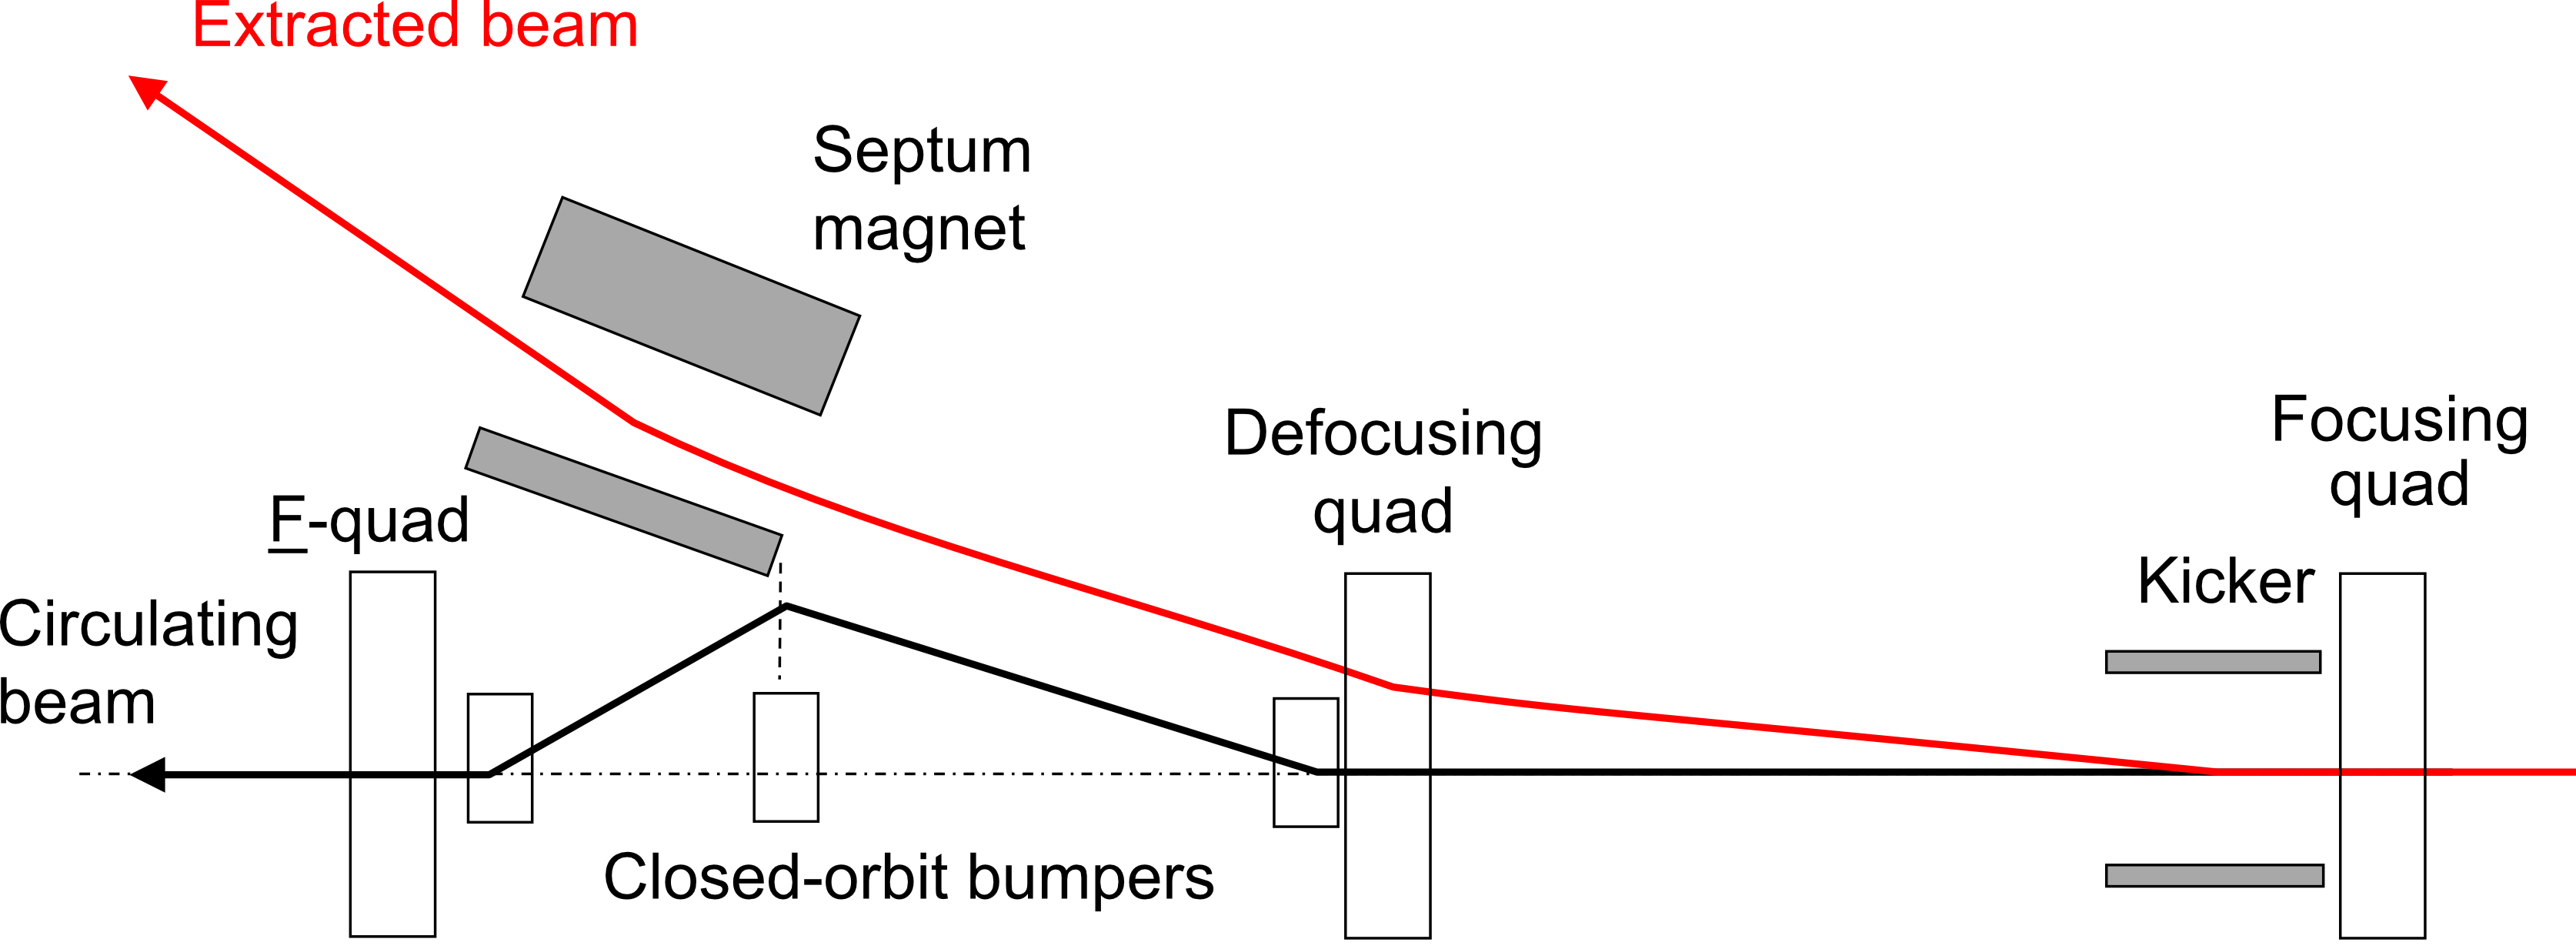
\includegraphics[width=\linewidth]{fast.png}
  \caption{Diagram of a general single-turn fast extraction system.~\cite{Fraser:CAS}}
  \label{fig:fast_diagram}
\end{figure}

This general method of \textbf{\textit{single-turn} fast extraction} (described in~\autoref{fig:fast_diagram}) is performed at two locations in the SPS---Long Straight Sections (LSS) 4 and 6---to fill the two counter-rotating beamlines in the LHC~\cite{Fraser:CAS}. The PSB performs similar extraction, but has the added complexity of ``merging'' four seperate stacked accelerators to one transfer line~\cite{Metzmacher:2061508}. LEIR likewise performs fast extraction~\cite{Ghithan:2017wpd}. The general layout of these systems are shown in~\ref{fig:chain}, where red diamonds mark fast extraction locations. Fast extraction systems are also used at the beam dump facilities at various stages of the accelerator chain.

In accelerator-to-accelerator contexts, the synchronous nature of fast extraction allows particles to remain bunched.~\textbf{Multi-turn fast extraction} extends this benefit, and is performed when filling the SPS for its fixed-target experiments (North Area) from the PS. As the SPS (\qty{6.9}{km}) is almost approximately 11 times longer in circumference than the PS\footnote{The PS is 100 meters across, and therefore $200\pi$\si{m}} (\qty{628}{m}), the entire SPS can be filled by 11 successive extractions of the full PS. This method, coined as \textit{continuous transfer} (CT), introduces the concept of ``shaving'' the beam with an electrostatic septum. In its current implementation in the PS, the beam is bumped similarly to single-turn fast extraction, but is instead forced over the blade of an electrostatic septum (ES), such that a segment the beam is `sliced' off, kicked towards a magnetic septum (MS), and extracted. The remaining beam is kicked back onto its orbit. The next turn, the beam has been ``rotated'' by a quarter turn, and the process repeats, until the finally the remaining core of the beam is bumped directly to the magnetic septum. This provides a spill to the SPS of five bunches over five beam rotations from a single PS bunch.

\begin{figure}[hb]
  \centering
  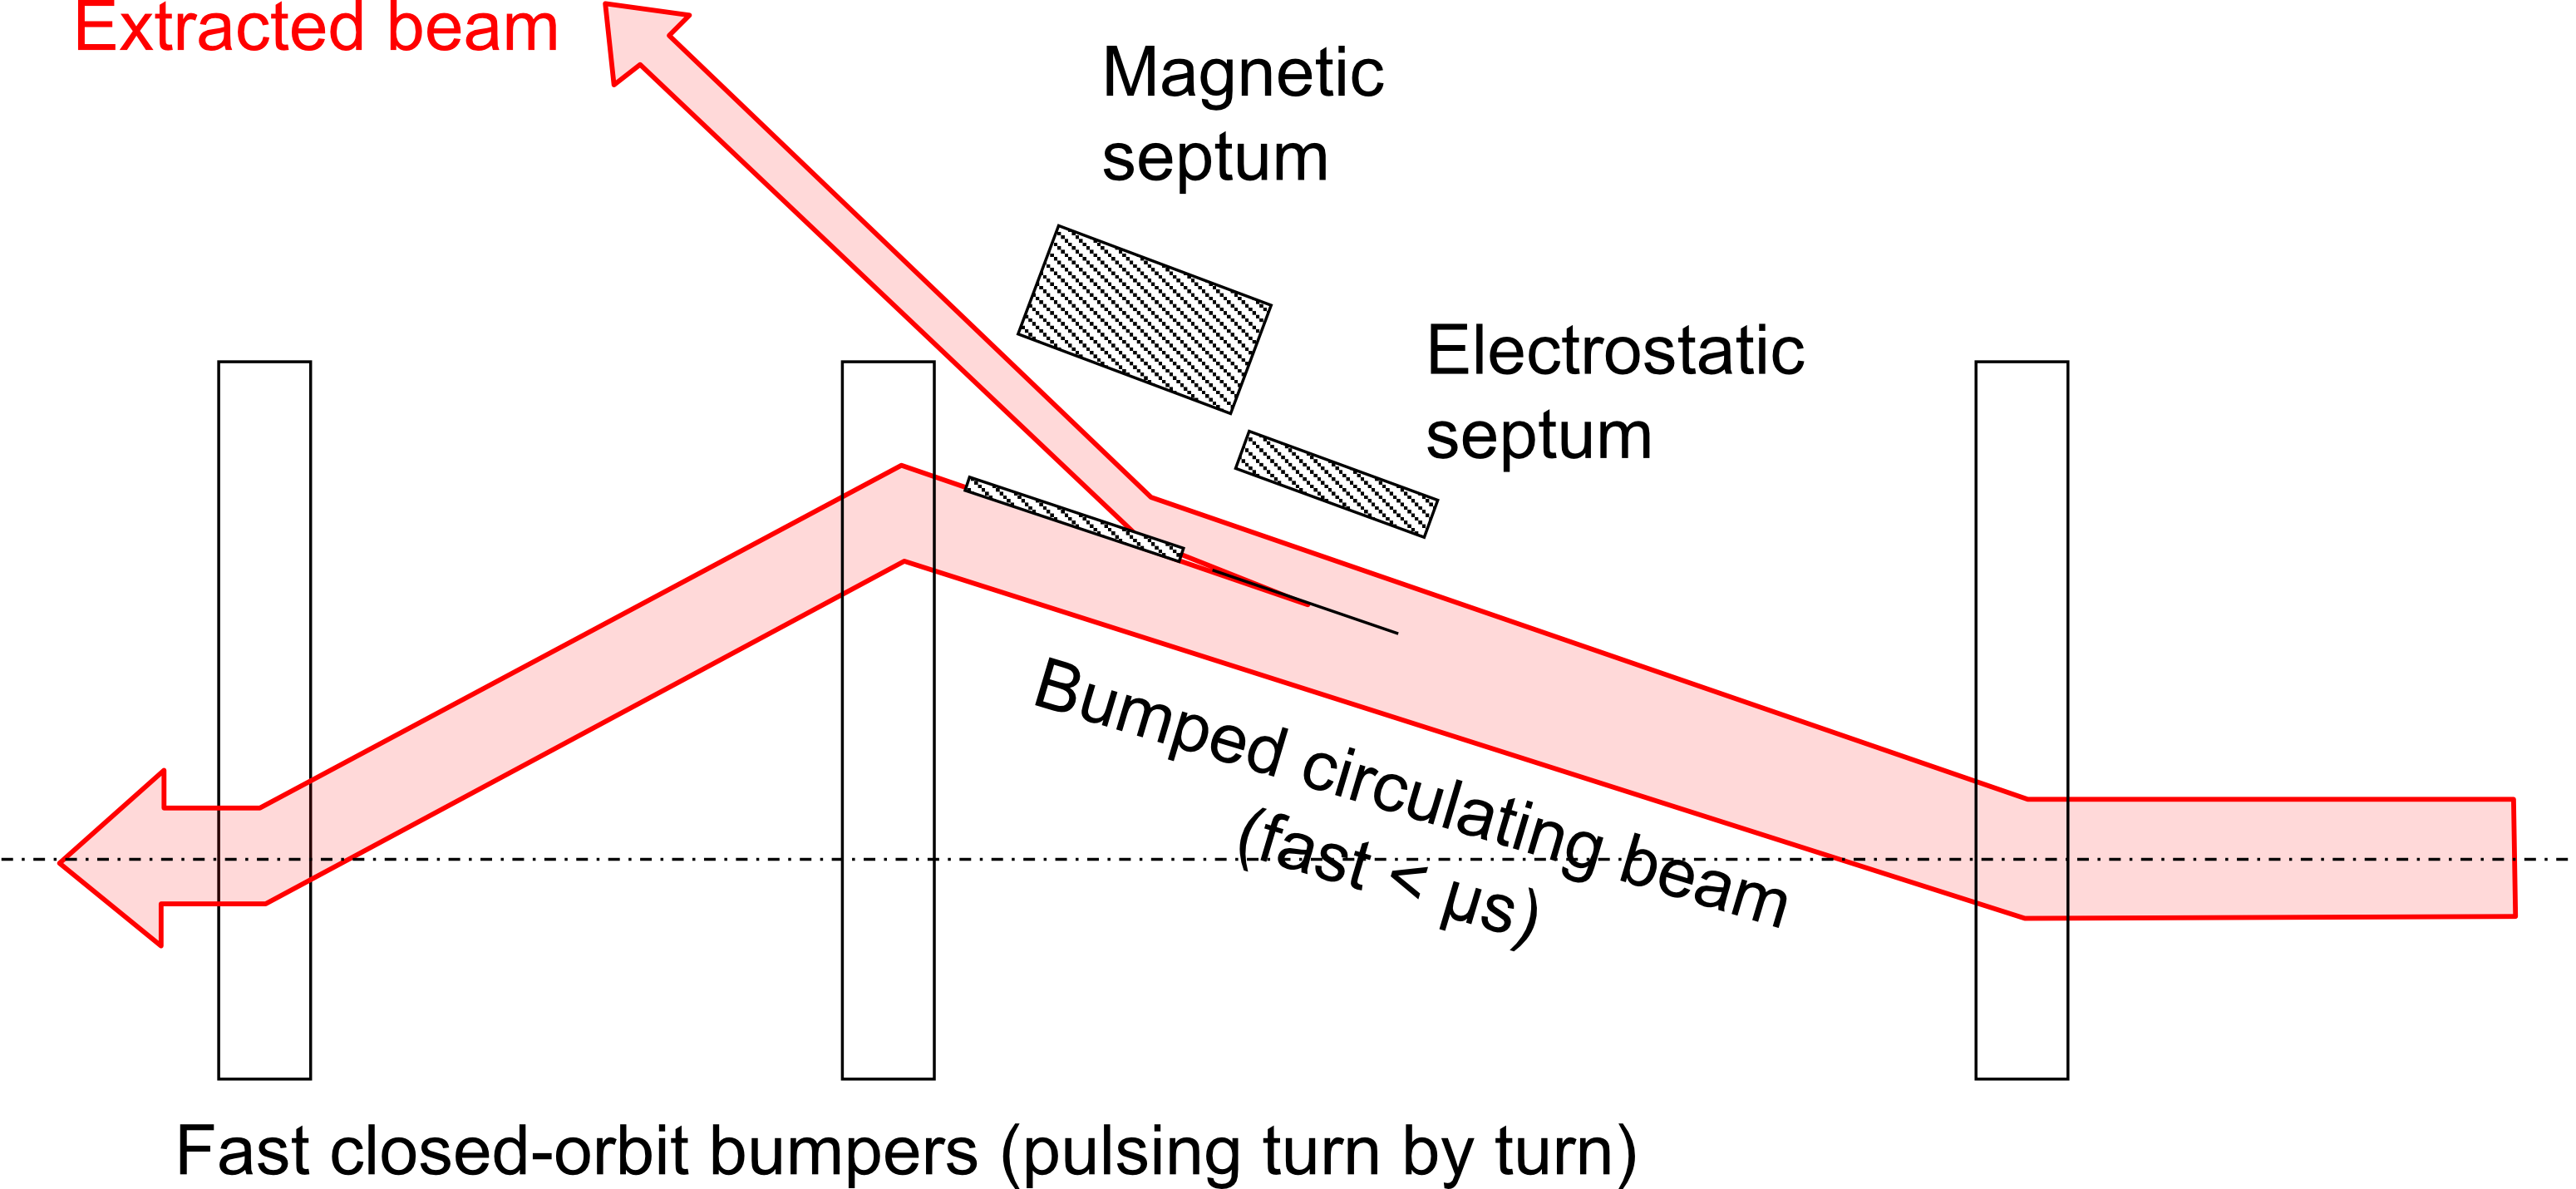
\includegraphics[width=\linewidth]{fastmulti.png}
  \caption{Diagram of a general multi-turn fast extraction system.~\cite{Fraser:CAS}}
  \label{fig:fast_multi_diagram}
\end{figure}

This method of increasing the spill time is, however, limited by the width of the septum blades. As the amount of beam scraped off per turn decreases, the effect of the particles lost \textit{on} the septum blade increases. To maintain a reasonable extraction efficiency, the beam size would have to become exponentially large.

For example, if a 50\% extraction efficiency is desired over $10^4$ turns, the beam thickness sliced off by the ES must be the same as the thickness of the blade itself. For the SPS, the ES has blade thickness of \qty{25}{\micro\meter}. The required diameter of the beam, therefore, would be $2\cdot 25\mu m\cdot 10^4 = $ \qty{0.5}{\meter}. This diameter is already lager than the beam pipes, clearly physically impossible.

In order to provide spills over a longer duration, approaching many thousands of turns, \textit{slow extraction} must be used. 

\subsection{Performing Slow Extraction}

\textbf{Slow extraction (SX)} instead relies on exploiting resonance of the beam as it oscillates around the orbit of the machine. A full theoretical description of these effects will be detailed in \autoref{chap:theory}, but a brief explanation is offered here: the oscillatory motion of a beam can be controlled such that it returns to the same point along the accelerators circumference with the same oscillation phase. The particles will, therefore, travel through the same field of a magnet, and experience the same force on successive turns. Akin to a child pushed on a swing in time with the peak of their oscillation, these particles will rapidly become unstable, the amplitude of their oscillations exponentially increasing. 

This resonant effect is usually carefully avoided in particle accelerators. However, with the right configuration, this amplitude growth can be used instead of an ES to separate particles from their orbit, towards an MS, and into the extraction transfer line. Should the effect be slow enough, a tiny fraction of particles will reach the MS per turn, and with a large enough per-turn amplitude growth to reliably clear the blade thickness.

The exploitation of resonance to induce extraction is by no means novel; a method akin to slow extraction was first proposed by J. Tuck and L. Teng in 1951~\cite{Couteur_1951}, and performed by Le Couteur at the Liverpool cyclotron in 1954~\cite{Couteur_1955}. Many such applications of slow extraction exist, using different effects to drive particles into resonance. This thesis will explore some of these methods, particularly focussing on Radio-Frequency Knockout slow extraction.

\subsection{Simulating Slow Extraction}

There are many applications for slow extraction systems beyond those currently used at CERN's experimental areas. Many medical synchrotrons, such as the MedAustron Synchrotron, use slow extraction to deliver beam to patients for ion beam cancer therapy~\cite{ArrutiaSota:2845862}. Using the \textit{Constant Optics Slow Extraction} (COSE) technique, spills of up to \qty{30}{\second} can be produced\footnote{Limited to \qty{10}{\second} for patient treatment}.

Obviously, in human medical applications, safety is extremely important. Therefore, the slow extraction process must be fully understood. Ripples in the intensity of beam have to be carefully controlled in order to provide a steady, predictable irradiation dose to patients.

Small medical synchrotrons are usually afforded the benefit of being simpler\footnote{The PS contains 100 bending magnets along its circumference, as opposed to MedAustron's 16}, newer\footnote{The PS began operation in 1959, and is CERN's oldest accelerator still in operation. MedAustron was first certified in 2016.}, and having less demand for availability than larger research synchrotrons such as the PS. At such machines, extensive machine tests can be carried out to fully understand the extraction process. At CERN's PS, however, that benefit cannot be relied upon. Availability is in high demand, and studies are time-shared between machine development (MD), fixed-target experimental areas, LHC physics injection, and a wide array of other facilities. 

Simulations can there provide a important tool in understanding slow extraction spills. New methods can be rapidly developed and tested without requiring extensive machine studies, and wide parameter spaces can be explored to construct functional relationships between input parameters and spill output characteristics. 

\section{Challenges}

Simulations for fast extraction are well understood; as explained later in \autoref{chap:theory}, the dynamics of particles in a ``static''\footnote{Static referring to the magnets and RF systems (known as the ``optics'' of the machine) being constant over the given time period.} machine can be understood with simple matrix transformations. However, many slow extraction methods rely on dynamic machines---the aforementioned COSE technique, despite its name, is not performed on a static machine, but instead scales the strength of magnets with the change in particle momentum, creating \textit{effectively} constant optics. Therefore, for each successive turn around the machine, the transport matrices must be re-calculated. For a typical slow extraction time of \qty{500}{\milli\second} at the PS, this equates to \qty{\approx235000}{turns}, and orders of magnitudes more calculations.

There are long-standing, well-tested tools for computing these transfer matrices for particle accelerators, which describe the motion of a particle---or ensemble of particles---as it travels through the accelerator, encountering different magnetic and electric fields.

To aid with the design and construction of CERN's Large Electron-Positron collider (LEP, the predecessor to LHC), the \textit{Methodical Accelerator Design Program} (MAD)~\cite{Iselin:MAD} was developed. This FORTRAN-based scripting tool allowed physicists to define the arrangement and strengths of magnetic elements around an accelerator (the \textit{lattice}), define beam parameters and initial conditions, and calculate the resulting motion of particles (the \textit{optics}). MAD, and its latest version, \verb|MAD-X|, quickly became the \textit{de facto} standard amongst particle accelerator institutions across the globe. However, in the twenty years since the release of \verb|MAD-X|, the landscape of computational accelerator physics has become awash with a wide array of tools, codes, and standards, each with their own specialisations. 

One particular improvement found in many new simulation programs is ``ready-to-go'' General-Purpose Graphical Processing Unit (GPGPU) acceleration. GPUs are specialised hardware capable of performing highly optimised matrix and vector calculations, initially intended for vector-based ray-tracing calculations. Where typical Central Processing Units have a wide range of general-purpose, unspecialised instructions and circuitry, GPUs are designed to perform a small set of highly optimised instructions on large arrays of data. This makes them ideal for the matrix calculations required for particle accelerator simulations. Additionally, where a typical CPU may contain anywhere from 4 to 64 cores, GPUs can contain many thousands of cores, capable of performing \textit{embarassingly parallel}\footnote{An \textit{embarassingly parallelisable} problem requires almost no effort to be separated into a large number of independent tasks which can be calculated concurrently.} calculations many orders of magnitude faster than a CPU.

\chapter{Theory}\label{chap:theory}

To construct accurate simulations of slow extraction methods, one must first understand the fundamental theory behind particle motion in a circular accelerator. This chapter will introduce the theory required to understand the motion of ensembles of particles as they travel through an accelerator, and how such oscillatory motion can be exploited to perform slow extraction. For a more in-depth treatment of beam dynamics and accelerator physics, the reader is referred to Wiedmann's \textit{Introduction to Accelerator Physics}~\cite{Wiedemann}.
\section{Single-Particle Transverse Beam Dynamics}

\subsection{Coordinate System}

The coordinate systems used to describe the dynamic motion of particles in a particle accelerator such as the PS relies on the periodic nature of a circular accelerator. Using a traditional Cartesian $x, y, z$ coordinate system would quickly introduce complications when describing circular trajectories, and so a local curvilinear coordinate system is used.

The basis vectors for this system, $(\hat x, \hat y, \hat s)$, constantly rotate in Cartesian space as the reference particle moves along the orbit of the accelerator. The longitudinal vector $\hat s$ is tangent to the particle's orbit, and the $\hat x$ direction is parallel to the radius of the accelerator. The absolute direction of $\hat y$ does not change, but makes one complete rotation in one closed orbit of the reference particle through the accelerator. This system is shown in Figure~\ref{fig:frenet-serret}, along with the radius of the circular trajectory $\rho$, and the angle from the origin $s=0$. 

\begin{figure}[!h]
\begin{center}
\tikzset{every picture/.style={line width=0.75pt}} %set default line width to 0.75pt        

\begin{tikzpicture}[x=0.75pt,y=0.75pt,yscale=-1,xscale=1]

%uncomment if require: \path (0,455); %set diagram left start at 0, and has height of 455

%Shape: Ellipse [id:dp0798878508534051] 
\draw   (142,162.5) .. controls (142,129.09) and (199.08,102) .. (269.5,102) .. controls (339.92,102) and (397,129.09) .. (397,162.5) .. controls (397,195.91) and (339.92,223) .. (269.5,223) .. controls (199.08,223) and (142,195.91) .. (142,162.5) -- cycle ;
%Straight Lines [id:da3917612889933506] 
\draw    (269.5,162.5) -- (269.5,57) ;
\draw [shift={(269.5,55)}, rotate = 90] [color={rgb, 255:red, 0; green, 0; blue, 0 }  ][line width=0.75]    (10.93,-3.29) .. controls (6.95,-1.4) and (3.31,-0.3) .. (0,0) .. controls (3.31,0.3) and (6.95,1.4) .. (10.93,3.29)   ;
%Straight Lines [id:da9587552919771436] 
\draw    (397,162.5) -- (269.5,162.5) ;
%Straight Lines [id:da15722891342539147] 
\draw    (269.5,162.5) -- (322.59,215.59) ;
\draw [shift={(324,217)}, rotate = 225] [color={rgb, 255:red, 0; green, 0; blue, 0 }  ][line width=0.75]    (10.93,-3.29) .. controls (6.95,-1.4) and (3.31,-0.3) .. (0,0) .. controls (3.31,0.3) and (6.95,1.4) .. (10.93,3.29)   ;
%Straight Lines [id:da7846346908558013] 
\draw    (324,217) -- (242.93,235.34) ;
\draw [shift={(240,236)}, rotate = 347.25] [fill={rgb, 255:red, 0; green, 0; blue, 0 }  ][line width=0.08]  [draw opacity=0] (10.72,-5.15) -- (0,0) -- (10.72,5.15) -- (7.12,0) -- cycle    ;
%Straight Lines [id:da569421074096844] 
\draw    (324,217) -- (324,141) ;
\draw [shift={(324,138)}, rotate = 90] [fill={rgb, 255:red, 0; green, 0; blue, 0 }  ][line width=0.08]  [draw opacity=0] (10.72,-5.15) -- (0,0) -- (10.72,5.15) -- (7.12,0) -- cycle    ;
%Straight Lines [id:da7806312488509295] 
\draw    (324,217) -- (345.88,238.88) ;
\draw [shift={(348,241)}, rotate = 225] [fill={rgb, 255:red, 0; green, 0; blue, 0 }  ][line width=0.08]  [draw opacity=0] (10.72,-5.15) -- (0,0) -- (10.72,5.15) -- (7.12,0) -- cycle    ;
%Curve Lines [id:da9180655893242637] 
\draw    (280,173) .. controls (284,177) and (291,162) .. (287,163) ;

% Text Node
\draw (406,153.4) node [anchor=north west][inner sep=0.75pt]    {$s=0$};
% Text Node
\draw (294,166.4) node [anchor=north west][inner sep=0.75pt]    {$\theta $};
% Text Node
\draw (271,177.4) node [anchor=north west][inner sep=0.75pt]    {$\rho $};
% Text Node
\draw (320,113.4) node [anchor=north west][inner sep=0.75pt]    {$\hat{y}$};
% Text Node
\draw (224,230.4) node [anchor=north west][inner sep=0.75pt]    {$\hat{s}$};
% Text Node
\draw (350,244.4) node [anchor=north west][inner sep=0.75pt]    {$\hat{x}$};


\end{tikzpicture}
\end{center}
\caption{The \textit{Frenet-Serret} vectors used to define the coordinate system used in particle beam dynamics.}\label{fig:frenet-serret}
\end{figure}

This coordinate system is academically known as a {\it Frenet-Serret} type coordinate system, and can be rigorously defined by the unit vector {\it tangent} to the curve $\hat T$ (pointing in the direction of motion), the unit vector {\it normal} to the tangent and on the tangential plane $\hat N$, and the binormal unit vector $\hat B$, the cross product of $\hat T$ and $\hat N$. These unit vectors, forming an orthonormal basis spanning $\mathbb{R}^3$, and known collectively as the {\bf TNB} frame, are equal to the vectors $\hat x, \hat y, \hat s$ by:
\begin{equation}
\begin{pmatrix}\hat T\\\hat N\\\hat B \end{pmatrix}=\begin{pmatrix}\hat s\\-\hat x\\\hat y \end{pmatrix}
\end{equation}

The coordinate system $(\hat x, \hat y, \hat s)$ relies on the right-hand chirality (Figure~\ref{fig:rhr}) of the vector cross product for the $\hat x$ vector to point radially outwards from the centre of the machine, the $\hat y$ vector points upwards, and the $\hat s$ vector points in the direction of motion. The direction of $\hat x$ to point outwards from the centre of revolution is chosen as injection and extraction line apertures will therefore be located in the positive $\hat x$.

\begin{figure}[!h]
\begin{center}
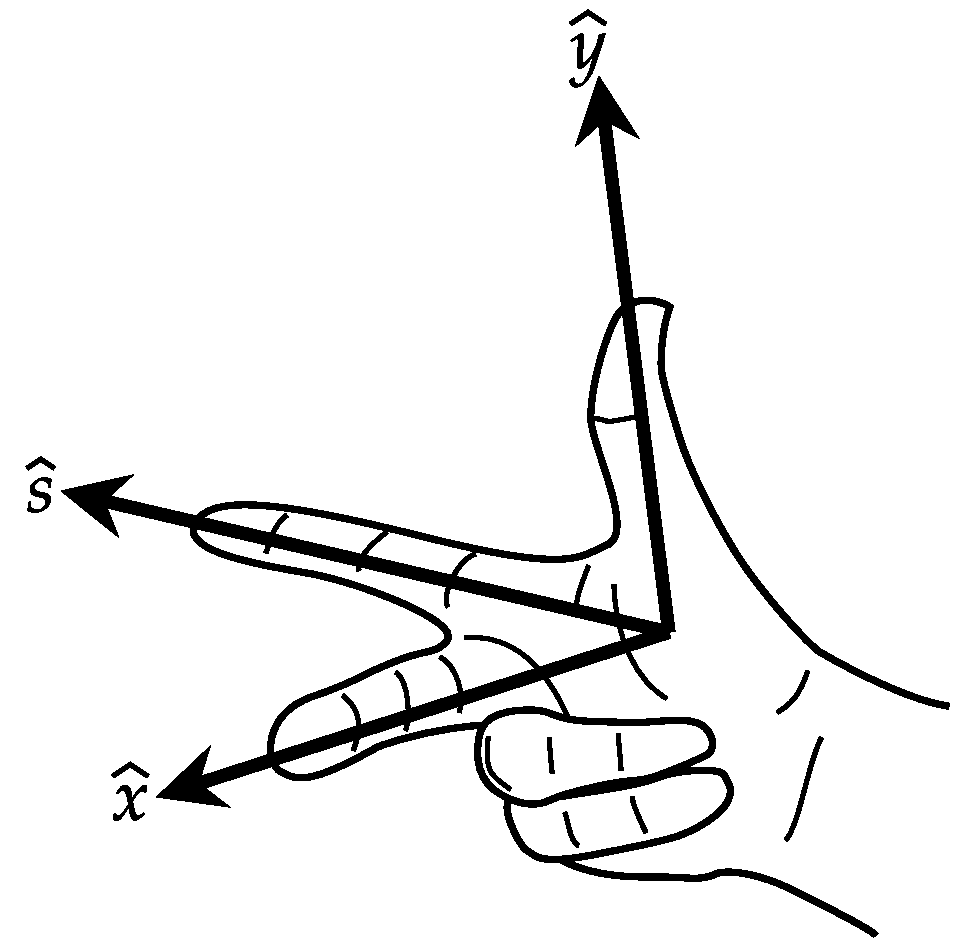
\includegraphics[scale=.25]{rhr.pdf}
\caption{The right-hand chirality rule defining the direction of $\hat x = \hat y \times \hat s$}
\label{fig:rhr}
\end{center}
\end{figure}

\subsection{Orbital Variable Space}

Following the basis vectors defining the coordinate system, the following variables are used to characterise the orbit of particles, dependent on $s$:
\begin{itemize}
  \item $x(s)$ [m]~---~the particle's horizontal position with respect to the reference orbit.
  \item $y(s)$ [m]~---~the particle's vertical position with respect to the reference orbit.
  \item $t(s)=-c\Delta t$ [m]~---~the particle's arrival delay with respect to the reference orbit, multiplied by the speed of light $c$.
  \item $x'(s)=\frac{dx}{ds}$ [rad]~---~the particle's horizontal angle with respect to the reference orbit.
  \item $y'(s)=\frac{dy}{ds}$ [rad]~---~the particle's vertical angle with respect to the reference orbit.
  \item $p_t(s)=\Delta E/pc$~---~the particle's energy difference, divided by the reference momentum times the speed of light $c$.
\end{itemize}

These variables provide a 6-tuple fully describing the trajectory of a particle. However, for the remainder of this thesis, the pair longitudinal variables $t, p_t$ will be treated separately to the transverse variable pairs $(x, x')$ and $(y, y')$. This enables a simpler understanding of the effects of beam bending and focussing magnets, as these effects are independent of the longitudinal variables. Conversely, longitudinal beam dynamics requires understanding or RF devices.

\subsection{Design orbit and Dipoles}

All descriptions of particle accelerators are build upon the Lorentz force, describing the force $\vec F$ acting on a charged particle with charge $q$ as it moves through an electric field $\vec E$ and magnetic field $\vec B$ with velocity $\vec v$, given as
\begin{equation}
\vec F_{\text{lorentz}} = q\cdot(\vec E+ \vec v\times\vec B)\label{eq:lorentz}
\end{equation}
This equation can already show why magnetic fields are used in almost all areas of particle acceleration, and not electric fields; a particle with higher velocity $v$ will experience a greater force from a constant magnetic field $\vec B$, whereas the contribution from the electric field $\vec E$ will remain constant. Therefore, at velocities approaching the speed of light ($v \rightarrow c$), we can begin to neglect $\vec E$ for some derivations.

The other force experienced by a particle in an accelerator is the centripetal\footnote{While the coordinate system used allows for a reference frame whose orientation follows the orbit, this frame is not co-moving with the particles, but still fixed in the ``laboratory'' frame---otherwise, complex Lorentz transformations would be required.} force:
\begin{equation}
\vec F_{\text{centrif.}}=\frac{m_0v^2}{\rho}\label{eq:centrifugal}
\end{equation} where $m_0$ is the particle's rest mass, and $\rho$ is the radius of the particle's orbit inside the accelerator.

Equating equations~\ref{eq:centrifugal} and~\ref{eq:lorentz} yields
\begin{equation}
B\rho=\frac pq
\end{equation}
The quantity $B\rho$ is known as the \textit{momentum rigidity} of a beam, and defines the bending angle of a particle for a given magnetic field. 

If the momentum $p=mv$ of the particle is measured in \unit[per-mode = symbol]{\GeV\per\clight\per amu}, and A and Ze are the atomic mass number and charge of the particle, the momentum rigidity can be expressed in Tesla-meters:

\begin{equation}
B\rho\ \left[\unit{\tesla\meter}\right]=\frac pq=\frac AZ\times3.33564\times q\ \left[\unit[per-mode=symbol]{\GeV\per\clight\per\atomicmassunit}\right]
\end{equation}

However, this formulation only describes a single magnetic field. In order to bend the particles along a circular trajectory, dipole magnets are used to create near-constant fields through which the particles travel. Again referring to~\autoref{eq:lorentz} (with the help of~\autoref{fig:rhr}), a magnetic field pointed vertically upwards (along the $\hat y$ vector) will cause a particle with motion along the $\hat s$ vector to experience a bending force along the $-\hat x$ direction (illustrated in~\autoref{fig:dipole}).

The arrangements of these bending magnets---referred to as Main Units (MU)---will define the closed loop of one orbit in the accelerator---the {\it design orbit}.

\begin{figure}[h]
  \centering

  \tikzset{every picture/.style={line width=0.75pt}} %set default line width to 0.75pt        

  \begin{tikzpicture}[x=0.75pt,y=0.75pt,yscale=-1,xscale=1]
  %uncomment if require: \path (0,420); %set diagram left start at 0, and has height of 420
  
  %Shape: Rectangle [id:dp3699492063250047] 
  \draw   (100,70) -- (250,70) -- (250,130) -- (100,130) -- cycle ;
  %Curve Lines [id:da992200965639283] 
  \draw [line width=2.25]    (90,100) .. controls (139.78,99.61) and (233.94,90.96) .. (286.81,71.22) ;
  \draw [shift={(290,70)}, rotate = 158.46] [color={rgb, 255:red, 0; green, 0; blue, 0 }  ][line width=2.25]    (17.49,-5.26) .. controls (11.12,-2.23) and (5.29,-0.48) .. (0,0) .. controls (5.29,0.48) and (11.12,2.23) .. (17.49,5.26)   ;
  %Shape: Rectangle [id:dp8960939916911084] 
  \draw   (320,70) -- (390,70) -- (390,130) -- (320,130) -- cycle ;
  %Shape: Rectangle [id:dp004915718994831897] 
  \draw   (320,60) -- (390,60) -- (390,70) -- (320,70) -- cycle ;
  %Shape: Rectangle [id:dp9834216786415646] 
  \draw   (320,130) -- (390,130) -- (390,140) -- (320,140) -- cycle ;
  %Straight Lines [id:da9215546463069324] 
  \draw    (330,83) -- (330,120) ;
  \draw [shift={(330,80)}, rotate = 90] [fill={rgb, 255:red, 0; green, 0; blue, 0 }  ][line width=0.08]  [draw opacity=0] (8.93,-4.29) -- (0,0) -- (8.93,4.29) -- cycle    ;
  %Straight Lines [id:da4829295704205643] 
  \draw    (380,83) -- (380,120) ;
  \draw [shift={(380,80)}, rotate = 90] [fill={rgb, 255:red, 0; green, 0; blue, 0 }  ][line width=0.08]  [draw opacity=0] (8.93,-4.29) -- (0,0) -- (8.93,4.29) -- cycle    ;
  %Straight Lines [id:da5246257542758568] 
  \draw    (355,83) -- (355,120) ;
  \draw [shift={(355,80)}, rotate = 90] [fill={rgb, 255:red, 0; green, 0; blue, 0 }  ][line width=0.08]  [draw opacity=0] (8.93,-4.29) -- (0,0) -- (8.93,4.29) -- cycle    ;
  %Straight Lines [id:da3445329346880859] 
  \draw  [dash pattern={on 4.5pt off 4.5pt}]  (90,100) -- (290,100) ;
  %Straight Lines [id:da3150179528223387] 
  \draw    (290,100) -- (290,73) ;
  \draw [shift={(290,70)}, rotate = 90] [fill={rgb, 255:red, 0; green, 0; blue, 0 }  ][line width=0.08]  [draw opacity=0] (8.93,-4.29) -- (0,0) -- (8.93,4.29) -- cycle    ;
  
  % Text Node
  \draw (334.5,42) node [anchor=north west][inner sep=0.75pt]   [align=left] {\begin{minipage}[lt]{29.38pt}\setlength\topsep{0pt}
  \begin{center}
  South
  \end{center}
  
  \end{minipage}};
  % Text Node
  \draw (336,141) node [anchor=north west][inner sep=0.75pt]   [align=left] {\begin{minipage}[lt]{27.66pt}\setlength\topsep{0pt}
  \begin{center}
  North
  \end{center}
  
  \end{minipage}};
  % Text Node
  \draw (361,84) node [anchor=north west][inner sep=0.75pt]   [align=left] {\begin{minipage}[lt]{9.78pt}\setlength\topsep{0pt}
  \begin{center}
  $\displaystyle \vec{B}$
  \end{center}
  
  \end{minipage}};
  % Text Node
  \draw (111,74) node [anchor=north west][inner sep=0.75pt]   [align=left] {\begin{minipage}[lt]{8.67pt}\setlength\topsep{0pt}
  \begin{center}
  $\displaystyle \vec{I}$
  \end{center}
  
  \end{minipage}};
  % Text Node
  \draw (292,73) node [anchor=north west][inner sep=0.75pt]   [align=left] {\begin{minipage}[lt]{9.14pt}\setlength\topsep{0pt}
  \begin{center}
  $\displaystyle \vec{F}$
  \end{center}
  
  \end{minipage}};
  % Text Node
  \draw (153,42) node [anchor=north west][inner sep=0.75pt]   [align=left] {\begin{minipage}[lt]{31.64pt}\setlength\topsep{0pt}
  \begin{center}
  Dipole
  \end{center}
  
  \end{minipage}};
  % Text Node
  \draw (123.5,171) node [anchor=north west][inner sep=0.75pt]   [align=left] {Top-down View};
  % Text Node
  \draw (311,172) node [anchor=north west][inner sep=0.75pt]   [align=left] {Front-on View};
  
  
  \end{tikzpicture}
  
  \caption{A dipole magnet, showing the direction of the magnetic field, $\vec B$, the current of the particle, $\vec I$, and the force, $\vec F$, on a positively charged particle.}\label{fig:dipole}
\end{figure}

If $\alpha$ is the bending angle of a single MU, then $\alpha$ can be related to the momentum rigidity by
\begin{equation}
\alpha=\frac{ds}\rho=\frac{B\ ds}{B\rho}
\end{equation}
Integrating this over all magnets in the ring, therefore, must be equal to one full revolution, $2\pi$
\begin{equation}
\frac{\int B\ ds}{B\rho}\equiv2\pi
\end{equation}

This provides one of the first key insights which is not obvious at first---that ``circular'' accelerators are in fact n-sided polygons, with bending magnets at each vertex, and a \textit{drift} (accelerator sections without any significant electromagnetic field) or other non-bending multipole magnet at each side: in the case of the LHC, 1,232 dipole magnets are used to keep the beam on it's circular path; in the PS---100.

\subsection{Focussing and Multipoles}

\begin{figure}[h]
\centering
\tikzset{every picture/.style={line width=0.75pt}} %set default line width to 0.75pt        
\begin{tikzpicture}[x=0.75pt,y=0.75pt,yscale=-1,xscale=1]
%uncomment if require: \path (0,420); %set diagram left start at 0, and has height of 420

%Shape: Rectangle [id:dp3699492063250047] 
\draw   (106.67,86.67) -- (340,86.67) -- (340,180) -- (106.67,180) -- cycle ;
%Curve Lines [id:da992200965639283] 
\draw [line width=2.25]    (90,133.33) .. controls (167.84,132.72) and (314.32,132.06) .. (396.3,101.42) ;
\draw [shift={(400,100)}, rotate = 158.46] [color={rgb, 255:red, 0; green, 0; blue, 0 }  ][line width=2.25]    (17.49,-5.26) .. controls (11.12,-2.23) and (5.29,-0.48) .. (0,0) .. controls (5.29,0.48) and (11.12,2.23) .. (17.49,5.26)   ;
%Straight Lines [id:da3445329346880859] 
\draw  [dash pattern={on 4.5pt off 4.5pt}]  (90,133.33) -- (401.11,133.33) ;
%Curve Lines [id:da8425102023911335] 
\draw [line width=2.25]    (88.89,126.67) .. controls (167.12,126.05) and (323.63,134.43) .. (397.78,52.51) ;
\draw [shift={(400,50)}, rotate = 130.87] [color={rgb, 255:red, 0; green, 0; blue, 0 }  ][line width=2.25]    (17.49,-5.26) .. controls (11.12,-2.23) and (5.29,-0.48) .. (0,0) .. controls (5.29,0.48) and (11.12,2.23) .. (17.49,5.26)   ;
%Flowchart: Summing Junction [id:dp8608620230880479] 
\draw   (116,103) .. controls (116,99.13) and (119.13,96) .. (123,96) .. controls (126.87,96) and (130,99.13) .. (130,103) .. controls (130,106.87) and (126.87,110) .. (123,110) .. controls (119.13,110) and (116,106.87) .. (116,103) -- cycle ; \draw   (118.05,98.05) -- (127.95,107.95) ; \draw   (127.95,98.05) -- (118.05,107.95) ;
% Text Node
\draw (132,91) node [anchor=north west][inner sep=0.75pt]   [align=left] {$\displaystyle \vec{B}$};
% Text Node
\draw (409,122) node [anchor=north west][inner sep=0.75pt]   [align=left] {$\displaystyle x=0$};


\end{tikzpicture}
\caption{A top-down diagram of a dipole illustrating how small changes in the beam's position, $x$, are amplified by the bending effect of the magnet.}
\label{fig:dipole_error}
\end{figure}

\autoref{fig:dipole_error} illustrates the need for corrective elements in the beamline. If a particle is displaced slightly from the design orbit ($x=0$) before a dipole element (marked with a downwards magnetic field $\vec B$), the bending effect will be greater, and the particle will be displaced further from the design orbit after the dipole. 

To correct for this, synchrotrons use quadrupole elements to ``focus'' the beam in one transverse plane. An arrangement of four magnetic poles creates a field stronger at higher $|x|$ displacement, causing particles to be pulled back towards the design orbit. However, particles off-axis in the other transverse plane will be pushed further off-axis. To correct for this, a second quadrupole is placed further along in the beamline, with the magnetic poles arranged in the opposite orientation. This arrangement, known as a FODO lattice, is shown in \autoref{fig:quadrupole} (right).

\begin{figure}
\centering
\tikzset{every picture/.style={line width=0.75pt}} %set default line width to 0.75pt        
\begin{tikzpicture}[x=0.75pt,y=0.75pt,yscale=-1,xscale=1]
%uncomment if require: \path (0,300); %set diagram left start at 0, and has height of 300

%Shape: Rectangle [id:dp16895106513799774] 
\draw   (165.86,51.72) -- (208.28,94.14) -- (194.14,108.28) -- (151.72,65.86) -- cycle ;
%Shape: Rectangle [id:dp7670602245044726] 
\draw   (75.86,141.72) -- (118.28,184.14) -- (104.14,198.28) -- (61.72,155.86) -- cycle ;
%Shape: Rectangle [id:dp12217894090817283] 
\draw   (208.28,155.86) -- (165.86,198.28) -- (151.72,184.14) -- (194.14,141.72) -- cycle ;
%Shape: Rectangle [id:dp07589692725962705] 
\draw   (118.28,65.86) -- (75.86,108.28) -- (61.72,94.14) -- (104.14,51.72) -- cycle ;
%Curve Lines [id:da018342825147440456] 
\draw    (80,100) .. controls (88.56,113.58) and (88.29,136.15) .. (81.62,147.61) ;
\draw [shift={(80,150)}, rotate = 308.25] [fill={rgb, 255:red, 0; green, 0; blue, 0 }  ][line width=0.08]  [draw opacity=0] (8.93,-4.29) -- (0,0) -- (8.93,4.29) -- cycle    ;
%Curve Lines [id:da03259735785014195] 
\draw    (110,70) .. controls (123.98,76.99) and (145.42,74.17) .. (157.17,70.87) ;
\draw [shift={(160,70)}, rotate = 161.57] [fill={rgb, 255:red, 0; green, 0; blue, 0 }  ][line width=0.08]  [draw opacity=0] (8.93,-4.29) -- (0,0) -- (8.93,4.29) -- cycle    ;
%Curve Lines [id:da729590423325807] 
\draw    (89.2,96.6) .. controls (103.87,116.48) and (102.52,130.21) .. (90.54,151.28) ;
\draw [shift={(89.2,153.6)}, rotate = 300.51] [fill={rgb, 255:red, 0; green, 0; blue, 0 }  ][line width=0.08]  [draw opacity=0] (8.93,-4.29) -- (0,0) -- (8.93,4.29) -- cycle    ;
%Curve Lines [id:da08909499648653463] 
\draw    (96.2,89.6) .. controls (115.5,106) and (114.31,137.31) .. (98.03,158.35) ;
\draw [shift={(96.2,160.6)}, rotate = 310.6] [fill={rgb, 255:red, 0; green, 0; blue, 0 }  ][line width=0.08]  [draw opacity=0] (8.93,-4.29) -- (0,0) -- (8.93,4.29) -- cycle    ;
%Curve Lines [id:da4406082857174254] 
\draw    (184.42,100.04) .. controls (170.84,119.33) and (173.24,133.1) .. (186.2,154.6) ;
\draw [shift={(186.2,97.6)}, rotate = 127.04] [fill={rgb, 255:red, 0; green, 0; blue, 0 }  ][line width=0.08]  [draw opacity=0] (8.93,-4.29) -- (0,0) -- (8.93,4.29) -- cycle    ;
%Curve Lines [id:da930807564323026] 
\draw    (176.7,92.71) .. controls (158.78,110.22) and (161.37,141.44) .. (179.04,161.6) ;
\draw [shift={(179.04,90.6)}, rotate = 140.27] [fill={rgb, 255:red, 0; green, 0; blue, 0 }  ][line width=0.08]  [draw opacity=0] (8.93,-4.29) -- (0,0) -- (8.93,4.29) -- cycle    ;
%Curve Lines [id:da5120218997402282] 
\draw    (111.04,172.69) .. controls (130.22,159.71) and (143.94,162.15) .. (165.29,174.83) ;
\draw [shift={(108.29,174.63)}, rotate = 323.78] [fill={rgb, 255:red, 0; green, 0; blue, 0 }  ][line width=0.08]  [draw opacity=0] (8.93,-4.29) -- (0,0) -- (8.93,4.29) -- cycle    ;
%Curve Lines [id:da8390452720928254] 
\draw    (103.45,165.31) .. controls (121.22,147.77) and (154.92,149.37) .. (172.32,167.85) ;
\draw [shift={(101.32,167.61)}, rotate = 310.56] [fill={rgb, 255:red, 0; green, 0; blue, 0 }  ][line width=0.08]  [draw opacity=0] (8.93,-4.29) -- (0,0) -- (8.93,4.29) -- cycle    ;
%Curve Lines [id:da6235876089908017] 
\draw    (113.26,178.83) .. controls (130.38,174.41) and (148.87,172.99) .. (160.29,179.63) ;
\draw [shift={(110.29,179.63)}, rotate = 344.31] [fill={rgb, 255:red, 0; green, 0; blue, 0 }  ][line width=0.08]  [draw opacity=0] (8.93,-4.29) -- (0,0) -- (8.93,4.29) -- cycle    ;
%Curve Lines [id:da24851523512173146] 
\draw    (106.29,76.02) .. controls (126.22,89.93) and (139.95,88.6) .. (160.98,77.12) ;
\draw [shift={(163.29,75.83)}, rotate = 150.49] [fill={rgb, 255:red, 0; green, 0; blue, 0 }  ][line width=0.08]  [draw opacity=0] (8.93,-4.29) -- (0,0) -- (8.93,4.29) -- cycle    ;
%Curve Lines [id:da9241759818534776] 
\draw    (99.32,82.71) .. controls (115.79,101.04) and (149.72,100.86) .. (168.35,84.34) ;
\draw [shift={(170.32,82.48)}, rotate = 134.64] [fill={rgb, 255:red, 0; green, 0; blue, 0 }  ][line width=0.08]  [draw opacity=0] (8.93,-4.29) -- (0,0) -- (8.93,4.29) -- cycle    ;
%Curve Lines [id:da909413050316068] 
\draw    (191.13,103.88) .. controls (185.3,123.95) and (186.46,138.2) .. (192,151) ;
\draw [shift={(192,101)}, rotate = 107.47] [fill={rgb, 255:red, 0; green, 0; blue, 0 }  ][line width=0.08]  [draw opacity=0] (8.93,-4.29) -- (0,0) -- (8.93,4.29) -- cycle    ;
%Straight Lines [id:da22347636828081718] 
\draw    (52,124.8) -- (128,124.8) ;
\draw [shift={(130,124.8)}, rotate = 180] [color={rgb, 255:red, 0; green, 0; blue, 0 }  ][line width=0.75]    (10.93,-3.29) .. controls (6.95,-1.4) and (3.31,-0.3) .. (0,0) .. controls (3.31,0.3) and (6.95,1.4) .. (10.93,3.29)   ;
%Straight Lines [id:da5667501984477679] 
\draw    (142,124.8) -- (162.2,124.8) -- (218,124.8) ;
\draw [shift={(140,124.8)}, rotate = 0] [color={rgb, 255:red, 0; green, 0; blue, 0 }  ][line width=0.75]    (10.93,-3.29) .. controls (6.95,-1.4) and (3.31,-0.3) .. (0,0) .. controls (3.31,0.3) and (6.95,1.4) .. (10.93,3.29)   ;
%Straight Lines [id:da690213494533449] 
\draw    (135,119.8) -- (135,46.6) ;
\draw [shift={(135,44.6)}, rotate = 90] [color={rgb, 255:red, 0; green, 0; blue, 0 }  ][line width=0.75]    (10.93,-3.29) .. controls (6.95,-1.4) and (3.31,-0.3) .. (0,0) .. controls (3.31,0.3) and (6.95,1.4) .. (10.93,3.29)   ;
%Straight Lines [id:da4326059970165157] 
\draw    (135,128.8) -- (135,207.6) ;
\draw [shift={(135,209.6)}, rotate = 270] [color={rgb, 255:red, 0; green, 0; blue, 0 }  ][line width=0.75]    (10.93,-3.29) .. controls (6.95,-1.4) and (3.31,-0.3) .. (0,0) .. controls (3.31,0.3) and (6.95,1.4) .. (10.93,3.29)   ;
%Shape: Ellipse [id:dp34626752560776697] 
\draw   (340.2,124) .. controls (340.2,104.12) and (344.63,88) .. (350.1,88) .. controls (355.57,88) and (360,104.12) .. (360,124) .. controls (360,143.88) and (355.57,160) .. (350.1,160) .. controls (344.63,160) and (340.2,143.88) .. (340.2,124) -- cycle ;
%Straight Lines [id:da6277807791700993] 
\draw [line width=2.25]    (350,100) -- (526.15,148.93) ;
\draw [shift={(530,150)}, rotate = 195.52] [color={rgb, 255:red, 0; green, 0; blue, 0 }  ][line width=2.25]    (17.49,-5.26) .. controls (11.12,-2.23) and (5.29,-0.48) .. (0,0) .. controls (5.29,0.48) and (11.12,2.23) .. (17.49,5.26)   ;
%Shape: Path Data [id:dp6636836986240371] 
\draw   (430,160) .. controls (432.76,160) and (435,144.33) .. (435,125) .. controls (435,105.67) and (432.76,90) .. (430,90) -- (450,90) .. controls (447.24,90) and (445,105.67) .. (445,125) .. controls (445,144.33) and (447.24,160) .. (450,160) -- (430,160) -- cycle ;
%Shape: Ellipse [id:dp8228024181704114] 
\draw   (520,124) .. controls (520,104.12) and (524.43,88) .. (529.9,88) .. controls (535.37,88) and (539.8,104.12) .. (539.8,124) .. controls (539.8,143.88) and (535.37,160) .. (529.9,160) .. controls (524.43,160) and (520,143.88) .. (520,124) -- cycle ;
%Straight Lines [id:da023007468461673675] 
\draw [line width=2.25]    (320,110) -- (346.21,101.26) ;
\draw [shift={(350,100)}, rotate = 161.57] [color={rgb, 255:red, 0; green, 0; blue, 0 }  ][line width=2.25]    (17.49,-5.26) .. controls (11.12,-2.23) and (5.29,-0.48) .. (0,0) .. controls (5.29,0.48) and (11.12,2.23) .. (17.49,5.26)   ;
%Straight Lines [id:da4640302291959706] 
\draw [line width=2.25]    (530,150) -- (556.21,141.26) ;
\draw [shift={(560,140)}, rotate = 161.57] [color={rgb, 255:red, 0; green, 0; blue, 0 }  ][line width=2.25]    (17.49,-5.26) .. controls (11.12,-2.23) and (5.29,-0.48) .. (0,0) .. controls (5.29,0.48) and (11.12,2.23) .. (17.49,5.26)   ;
%Straight Lines [id:da879655645129539] 
\draw  [dash pattern={on 4.5pt off 4.5pt}]  (312.8,125) -- (568.8,125) ;

% Text Node
\draw (84,72) node [anchor=north west][inner sep=0.75pt]   [align=left] {N};
% Text Node
\draw (175,162) node [anchor=north west][inner sep=0.75pt]   [align=left] {N};
% Text Node
\draw (175,71) node [anchor=north west][inner sep=0.75pt]   [align=left] {S};
% Text Node
\draw (85,163) node [anchor=north west][inner sep=0.75pt]   [align=left] {S};
% Text Node
\draw (223,111) node [anchor=north west][inner sep=0.75pt]   [align=left] {$\displaystyle \vec{F}$};
% Text Node
\draw (331,62) node [anchor=north west][inner sep=0.75pt]   [align=left] {Focus};
% Text Node
\draw (412,62) node [anchor=north west][inner sep=0.75pt]   [align=left] {Defocus};
% Text Node
\draw (511,62) node [anchor=north west][inner sep=0.75pt]   [align=left] {Focus};
\end{tikzpicture}
\caption{Diagram (left) showing the field of a \textit{normal} oriented quadrupole, providing focussing in $x$ but defocussing in $y$. Right-hand diagram illustrates a FODO cell.}
\label{fig:quadrupole}
\end{figure}

Sextupoles---third order magnets---provide additional correction to the beam. Here, we can begin to expand on the optical analogy used thus far.~\autoref{fig:optics} shows a full arrangement of a dipole, sextupole, and focussing quadrupole. In the optical analogy, the Dipole takes the role of a prism, bending the light. As with prisms, beams with higher energy are bent less than low energy, and so the component wavelengths (or energies) in the beam beam are dispersed. The sextupole is analogous to an aspherical element, correcting for chromatic aberration introduced by the focussing quadrupole. Again, as with its optical analogue---a focussing lens---the quadrupole has shorter focal length for higher energy particles. The sextupole acts as a focussing lens at high energy and diverging lens at low energy, correcting for this chromatic effect.

\begin{figure}
\centering
\tikzset{every picture/.style={line width=0.75pt}} %set default line width to 0.75pt        
\begin{tikzpicture}[x=0.75pt,y=0.75pt,yscale=-1,xscale=1]
%uncomment if require: \path (0,420); %set diagram left start at 0, and has height of 420

%Straight Lines [id:da5032125547450867] 
\draw [color={rgb, 255:red, 0; green, 0; blue, 0 }  ,draw opacity=1 ][line width=2.25]    (20,250) -- (40,200) ;
%Straight Lines [id:da7193947806706618] 
\draw [color={rgb, 255:red, 74; green, 144; blue, 226 }  ,draw opacity=1 ][line width=2.25]    (210,170) -- (310,170) ;
%Straight Lines [id:da9130386432813542] 
\draw [color={rgb, 255:red, 0; green, 0; blue, 0 }  ,draw opacity=1 ][line width=2.25]    (40,250) -- (60,200) ;
%Straight Lines [id:da27606687123687523] 
\draw [color={rgb, 255:red, 208; green, 2; blue, 27 }  ,draw opacity=1 ][line width=2.25]    (310,70) -- (438.8,75.6) ;
%Flowchart: Preparation [id:dp23094783659480855] 
\draw   (290,130) -- (297.5,60) -- (322.5,60) -- (330,130) -- (322.5,200) -- (297.5,200) -- cycle ;
%Straight Lines [id:da18224121501659596] 
\draw [color={rgb, 255:red, 208; green, 2; blue, 27 }  ,draw opacity=1 ][line width=2.25]    (210,70) -- (310,70) ;
%Straight Lines [id:da07220877512576229] 
\draw [color={rgb, 255:red, 208; green, 2; blue, 27 }  ,draw opacity=1 ][line width=2.25]    (310,90) -- (439.8,88.6) ;
%Straight Lines [id:da4744481623787409] 
\draw [color={rgb, 255:red, 208; green, 2; blue, 27 }  ,draw opacity=1 ][line width=2.25]    (210,90) -- (310,90) ;
%Straight Lines [id:da7680471071414616] 
\draw [color={rgb, 255:red, 126; green, 211; blue, 33 }  ,draw opacity=1 ][line width=2.25]    (210,110) -- (310,110) ;
%Straight Lines [id:da7247321208701782] 
\draw [color={rgb, 255:red, 126; green, 211; blue, 33 }  ,draw opacity=1 ][line width=2.25]    (310,110) -- (440,110) ;
%Straight Lines [id:da28519750675372135] 
\draw [color={rgb, 255:red, 126; green, 211; blue, 33 }  ,draw opacity=1 ][line width=2.25]    (210,150) -- (440,150) ;
%Straight Lines [id:da8241694279527554] 
\draw [color={rgb, 255:red, 74; green, 144; blue, 226 }  ,draw opacity=1 ][line width=2.25]    (210,191) -- (310,191) ;
%Straight Lines [id:da6175125823498442] 
\draw [color={rgb, 255:red, 74; green, 144; blue, 226 }  ,draw opacity=1 ][line width=2.25]    (310,170) -- (439.2,175.6) ;
%Straight Lines [id:da5918352005930418] 
\draw [color={rgb, 255:red, 74; green, 144; blue, 226 }  ,draw opacity=1 ][line width=2.25]    (310,191) -- (440,200) ;
%Shape: Ellipse [id:dp03595429672574735] 
\draw   (430,130) .. controls (430,85.82) and (434.48,50) .. (440,50) .. controls (445.52,50) and (450,85.82) .. (450,130) .. controls (450,174.18) and (445.52,210) .. (440,210) .. controls (434.48,210) and (430,174.18) .. (430,130) -- cycle ;
%Straight Lines [id:da1814744582158785] 
\draw [color={rgb, 255:red, 208; green, 2; blue, 27 }  ,draw opacity=1 ][line width=2.25]    (439.8,88.6) -- (610,130) ;
%Straight Lines [id:da46080486956508504] 
\draw [color={rgb, 255:red, 208; green, 2; blue, 27 }  ,draw opacity=1 ][line width=2.25]    (438.8,75.6) -- (610,130) ;
%Straight Lines [id:da7978877411725234] 
\draw [color={rgb, 255:red, 126; green, 211; blue, 33 }  ,draw opacity=1 ][line width=2.25]    (440,110) -- (610,130) ;
%Straight Lines [id:da45611278933138877] 
\draw [color={rgb, 255:red, 126; green, 211; blue, 33 }  ,draw opacity=1 ][line width=2.25]    (440,150) -- (610,130) ;
%Straight Lines [id:da47306718166192696] 
\draw [color={rgb, 255:red, 74; green, 144; blue, 226 }  ,draw opacity=1 ][line width=2.25]    (439.2,175.6) -- (610,130) ;
%Straight Lines [id:da8057830718576857] 
\draw [color={rgb, 255:red, 74; green, 144; blue, 226 }  ,draw opacity=1 ][line width=2.25]    (440,200) -- (610,130) ;
%Shape: Ellipse [id:dp869139000293633] 
\draw   (305,82) .. controls (305,70.95) and (307.24,62) .. (310,62) .. controls (312.76,62) and (315,70.95) .. (315,82) .. controls (315,93.05) and (312.76,102) .. (310,102) .. controls (307.24,102) and (305,93.05) .. (305,82) -- cycle ;
%Shape: Path Data [id:dp22450547395269504] 
\draw   (304,195) .. controls (305.38,195) and (306.5,188.28) .. (306.5,180) .. controls (306.5,171.72) and (305.38,165) .. (304,165) -- (314,165) .. controls (312.62,165) and (311.5,171.72) .. (311.5,180) .. controls (311.5,188.28) and (312.62,195) .. (314,195) -- (304,195) -- cycle ;
%Curve Lines [id:da9020894578602425] 
\draw [color={rgb, 255:red, 208; green, 2; blue, 27 }  ,draw opacity=1 ][line width=2.25]    (40,200) .. controls (48.2,177.6) and (87.2,71.6) .. (210,70) ;
%Curve Lines [id:da8005791954562751] 
\draw [color={rgb, 255:red, 208; green, 2; blue, 27 }  ,draw opacity=1 ][line width=2.25]    (60,200) .. controls (74.2,176.6) and (83.2,96.6) .. (210,90) ;
%Curve Lines [id:da7337546567844901] 
\draw [color={rgb, 255:red, 126; green, 211; blue, 33 }  ,draw opacity=1 ][line width=2.25]    (40,200) .. controls (54.2,176.6) and (83.2,116.6) .. (210,110) ;
%Curve Lines [id:da37909296710645] 
\draw [color={rgb, 255:red, 126; green, 211; blue, 33 }  ,draw opacity=1 ][line width=2.25]    (60,200) .. controls (74.2,176.6) and (83.2,156.6) .. (210,150) ;
%Curve Lines [id:da1812313073325389] 
\draw [color={rgb, 255:red, 74; green, 144; blue, 226 }  ,draw opacity=1 ][line width=2.25]    (40,200) .. controls (68.2,164.6) and (147.2,169.6) .. (210,170) ;
%Curve Lines [id:da9550611143964061] 
\draw [color={rgb, 255:red, 74; green, 144; blue, 226 }  ,draw opacity=1 ][line width=2.25]    (60,200) .. controls (62.2,192.6) and (149.2,189.6) .. (210,191) ;
%Straight Lines [id:da7770063556142277] 
\draw    (210,60) -- (100,220) ;
%Straight Lines [id:da5255637367733044] 
\draw    (30,60) -- (10,220) ;
%Straight Lines [id:da8889577051375981] 
\draw    (210,60) -- (30,60) ;
%Straight Lines [id:da09835929734762772] 
\draw    (100,220) -- (10,220) ;

% Text Node
\draw (81,32) node [anchor=north west][inner sep=0.75pt]   [align=left] {Dipole};
% Text Node
\draw (278,32) node [anchor=north west][inner sep=0.75pt]   [align=left] {Sextupole};
% Text Node
\draw (401,32) node [anchor=north west][inner sep=0.75pt]   [align=left] {Quadrupole};
% Text Node
\draw (41,72) node [anchor=north west][inner sep=0.75pt]   [align=left] {{\small High-Energy}};
% Text Node
\draw (121,193) node [anchor=north west][inner sep=0.75pt]   [align=left] {{\small Low-Energy}};


\end{tikzpicture}
\caption{A diagram showing how Dipoles, Quadrupoles, and Sextupoles are used together to create the desired beam dynamics for particles with different energies.}
\label{fig:optics}
\end{figure}

%============================================================================================%

Now that the basic magnetic elements have been introduced, and an understanding of the beam's momentum $p$ has been formed, we can redefine our transverse coordinates in terms of momentum: $p_x=x'\cdot p$ and $p_y=y'\cdot p$ now define our transverse coordinates. These coordinates will allow us to build a picture of the multi-particle transverse dynamics of the beam.

\subsection{Single-Particle Oscillatory Motion}

% In the transverse dynamics of an accelerated beam, the {\it betatron function} refers to one of the three functions ($\alpha$, $\beta$, and $\gamma$), which, along with betatron phase $\mu$, can provide an emittance-independent representation of the properties of the beam. These functions are known as the {\it Twiss} or {\it Courant-Snyder} parameters of a transverse dynamics system. 


In a periodic (circular) accelerator, the linear equation for transverse motion takes the form of a differential equation:

\begin{equation}
  x''(s)-x\cdot\left(k-\frac{1}{\rho^2}\right)=0
  \label{eq:diff_motion}
\end{equation} 
where $x$ is the transverse displacement as a function of longitudinal position $s$, and $k$ is the quadrupole focussing coefficient, defined as
\begin{equation}
  k=\frac{q}{p}\cdot\frac{dB_y}{dx}
  \label{eq:quadrupole}
\end{equation} where $q$ is the particle's charge, $p$ is the longitudinal momentum, and $B_y$ is the vertical component of the magnetic field. The $1/\rho^2$ term represents the effect of the dipole bending field, providing a weak focussing component.
From here, it is clear that the transverse motion of particles, in a circular accelerator and under the influence of dipole focussing $1/\rho^2$ and quadrupole focussing $k$, follows a harmonic oscillator. If we enforce the periodicity\footnote{i.e. that the quadrupoles do not change between successive revolutions} in $s$ of $k$, Equation~\ref{eq:diff_motion} can be rewritten in a compact form
\begin{equation}
  x''(s)-\tilde{k}(s)x(s)=0
  \label{eq:hill}
\end{equation} where the quadrupole focussing component $\tilde{k}(s)$ is now a function of $s$. With the given periodic boundary condition $\tilde k(s+L)=\tilde{k}(s)$,~\ref{eq:hill} is known as the Hill's equation. 

Following Floquet's theorem~\cite{Rossbach:247501}, general solution to this equation takes the form of
\begin{equation}
x(s) =\sqrt{\varepsilon}\sqrt{\beta(s)}\cos(\varphi(s)-\varphi_0)
\label{eq:motion_x}
\end{equation} where $\varepsilon$ and $\varphi_0$ are integration constants characterising the initial conditions of the particle, and $\beta(s)$ and $\varphi(s)$ are the amplitude and phase functions (respectively) of the oscillation.

The $\beta$ amplitude function must also satisfy the periodic constraint $\beta(s+L)=\beta(s)$, and can be related to the $\varphi$ phase function by the following equation:
\begin{eqnarray}
  \varphi(s) = \int^s_0\frac{ds}{\beta(s)}
  \label{eq:phase_and_beta}
\end{eqnarray}


Taking the derivative of~\eqref{eq:motion_x} with respect to $s$ gives an equation for the angle of the trajectory:
\begin{equation}
x'(s)=\sqrt{\varepsilon}\sqrt{\beta(s)}\left(\frac12\beta'(s)\cos(\varphi(s)-\varphi_0)+\sin(\varphi(s))\right)
\label{eq:motion_px}
\end{equation}

A basic analysis of~\eqref{eq:phase_and_beta} shows that at locations with large $\beta$ amplitude (and thus a large transverse displacement), phase advance $\varphi$ is small, and vice versa. The overall phase advance of transverse oscillations over one revolution of $2\pi$ is known as the \textit{betatron tune} of the accelerator, and is defined as
\begin{equation}
  Q=\frac12\oint\frac{ds}{\beta(s)}
  \label{eq:betatron_tune}
\end{equation}
This quantity, often simply referred to as \textit{tune}, effectively indicates how many complete transverse oscillations a particle makes in one turn. The fractional part of this value is the most significant, and often a tune will be reference to the integer part; a tune of $Q=6.\dot 3=19/3$ is, for the purposes of this thesis, equivalent to $Q=1/3$.
\clearpage

\section{Multi-Particle Transverse Beam Dynamics}\label{sec:theory-transverse}

\subsection{Phase Space}

\autoref{eq:motion_x} and~\autoref{eq:motion_px} introduced an integration constant $\varepsilon$, which is a characteristic parameter of the particle or ensemble of particles. It is known as (transverse) emittance, and is usually considered with particle ensembles in mind. These two equations can be manipulated to provide an expression for $\varepsilon$:
\begin{equation}
  \varepsilon = \gamma(s)x^2(s)+2\alpha x(s)x'(s)+\beta(s)x'^2(s)
  \label{eq:emittance}
\end{equation} where 
\begin{equation}
  \alpha(s) = -\frac12\frac{d\beta(s)}{ds}
  \label{eq:alpha}
\end{equation} and
\begin{eqnarray}
  \gamma(s) = \frac{1+\alpha^2(s)}{\beta(s)}
  \label{eq:gamma}
\end{eqnarray}

These further two constants, along with $\beta$, form the \textit{Courant-Snyder Parameters}~\cite{courantsnyder}, commonly referred to as the \textit{twiss} parameters\footnote{Even Richard Q. Twiss, a British astronomer, was himself unsure as to how the parameters became attributed to him~\cite{richardtwiss}.}. 

These parameters can be readily understood in the \textit{phase space}\footnote{This is opposed to the more formal phase space $(x, p_x)$, which does not provide these insights as succinctly.} of $(x, x')$. Illustrated in~\autoref{fig:twiss-phase-space}, \autoref{eq:emittance} describes an ellipse, which covers the area of the particle ensemble in phase space. The area of this ellipse is given by $\pi\cdot\varepsilon$, and may be interchangeably defined as the emittance. 

\begin{figure}[h]
  \centering
  \tikzset{every picture/.style={line width=0.75pt}} %set default line width to 0.75pt        
  \begin{tikzpicture}[x=0.75pt,y=0.75pt,yscale=-1,xscale=1]
  %uncomment if require: \path (0,300); %set diagram left start at 0, and has height of 300
  
  %Straight Lines [id:da9035065264450608] 
  \draw    (330,290) -- (330,12) ;
  \draw [shift={(330,10)}, rotate = 90] [color={rgb, 255:red, 0; green, 0; blue, 0 }  ][line width=0.75]    (10.93,-3.29) .. controls (6.95,-1.4) and (3.31,-0.3) .. (0,0) .. controls (3.31,0.3) and (6.95,1.4) .. (10.93,3.29)   ;
  %Straight Lines [id:da452302761105561] 
  \draw    (190,150) -- (468,150) ;
  \draw [shift={(470,150)}, rotate = 180] [color={rgb, 255:red, 0; green, 0; blue, 0 }  ][line width=0.75]    (10.93,-3.29) .. controls (6.95,-1.4) and (3.31,-0.3) .. (0,0) .. controls (3.31,0.3) and (6.95,1.4) .. (10.93,3.29)   ;
  %Shape: Ellipse [id:dp6041133983422828] 
  \draw   (407.78,72.22) .. controls (419.93,84.37) and (394.95,129.04) .. (352,172) .. controls (309.04,214.95) and (264.37,239.93) .. (252.22,227.78) .. controls (240.07,215.63) and (265.05,170.96) .. (308,128) .. controls (350.96,85.05) and (395.63,60.07) .. (407.78,72.22) -- cycle ;
  %Straight Lines [id:da2286251239967374] 
  \draw  [dash pattern={on 4.5pt off 4.5pt}]  (410,80) -- (410,260) ;
  %Straight Lines [id:da9188194183446701] 
  \draw    (350,250) -- (332,250) ;
  \draw [shift={(330,250)}, rotate = 360] [fill={rgb, 255:red, 0; green, 0; blue, 0 }  ][line width=0.08]  [draw opacity=0] (12,-3) -- (0,0) -- (12,3) -- cycle    ;
  %Straight Lines [id:da052944294077684084] 
  \draw    (390,250) -- (408,250) ;
  \draw [shift={(410,250)}, rotate = 180] [fill={rgb, 255:red, 0; green, 0; blue, 0 }  ][line width=0.08]  [draw opacity=0] (12,-3) -- (0,0) -- (12,3) -- cycle    ;
  %Straight Lines [id:da26164850536705697] 
  \draw  [dash pattern={on 4.5pt off 4.5pt}]  (400,70) -- (220,70) ;
  %Straight Lines [id:da5891228483681046] 
  \draw    (230,100) -- (230,72) ;
  \draw [shift={(230,70)}, rotate = 90] [fill={rgb, 255:red, 0; green, 0; blue, 0 }  ][line width=0.08]  [draw opacity=0] (12,-3) -- (0,0) -- (12,3) -- cycle    ;
  %Straight Lines [id:da503222730024451] 
  \draw    (230,120) -- (230,148) ;
  \draw [shift={(230,150)}, rotate = 270] [fill={rgb, 255:red, 0; green, 0; blue, 0 }  ][line width=0.08]  [draw opacity=0] (12,-3) -- (0,0) -- (12,3) -- cycle    ;
  %Straight Lines [id:da3735583359226975] 
  \draw  [dash pattern={on 4.5pt off 4.5pt}]  (430,50) -- (220,260) ;
  %Straight Lines [id:da030558782090539305] 
  \draw  [dash pattern={on 4.5pt off 4.5pt}]  (400,70) -- (400,30) ;
  %Straight Lines [id:da1130230393821896] 
  \draw    (332,50) -- (398,50) ;
  \draw [shift={(400,50)}, rotate = 180] [fill={rgb, 255:red, 0; green, 0; blue, 0 }  ][line width=0.08]  [draw opacity=0] (12,-3) -- (0,0) -- (12,3) -- cycle    ;
  \draw [shift={(330,50)}, rotate = 0] [fill={rgb, 255:red, 0; green, 0; blue, 0 }  ][line width=0.08]  [draw opacity=0] (12,-3) -- (0,0) -- (12,3) -- cycle    ;
  %Straight Lines [id:da9823091980720369] 
  \draw  [dash pattern={on 4.5pt off 4.5pt}]  (410,80) -- (460,80) ;
  %Straight Lines [id:da26364391504483] 
  \draw    (440,148) -- (440,82) ;
  \draw [shift={(440,80)}, rotate = 90] [fill={rgb, 255:red, 0; green, 0; blue, 0 }  ][line width=0.08]  [draw opacity=0] (12,-3) -- (0,0) -- (12,3) -- cycle    ;
  \draw [shift={(440,150)}, rotate = 270] [fill={rgb, 255:red, 0; green, 0; blue, 0 }  ][line width=0.08]  [draw opacity=0] (12,-3) -- (0,0) -- (12,3) -- cycle    ;
  
  % Text Node
  \draw (475,139) node [anchor=north west][inner sep=0.75pt]   [align=left] {$\displaystyle x$};
  % Text Node
  \draw (304,2) node [anchor=north west][inner sep=0.75pt]   [align=left] {$\displaystyle x'$};
  % Text Node
  \draw (352,237) node [anchor=north west][inner sep=0.75pt]   [align=left] {$\displaystyle \sqrt{\varepsilon \beta }$};
  % Text Node
  \draw (214,99) node [anchor=north west][inner sep=0.75pt]   [align=left] {$\displaystyle \sqrt{\varepsilon \gamma }$};
  % Text Node
  \draw (441,21.4) node [anchor=north west][inner sep=0.75pt]    {$\tan 2\theta =\frac{2\alpha }{\gamma -\beta }$};
  % Text Node
  \draw (331,11) node [anchor=north west][inner sep=0.75pt]   [align=left] {$\displaystyle -\alpha \sqrt{\nicefrac{\varepsilon}{\gamma}}$};
  % Text Node
  \draw (447,92) node [anchor=north west][inner sep=0.75pt]   [align=left] {$\displaystyle -\alpha \sqrt{\nicefrac{\varepsilon}{\beta}}$};
  % Text Node
  \draw (181,180) node [anchor=north west][inner sep=0.75pt]   [align=left] {$\displaystyle A=\pi \varepsilon $};
  
  
  \end{tikzpicture}
  \caption{Phase space in $(x, x')$ showing the ellipse formed by a particle, and its relation to the Twiss parameters.}
  \label{fig:twiss-phase-space}
\end{figure}

Liouville's theorem states that, under conservative forces, this emittance is conserved, and no external field can change it, and hence~\autoref{eq:motion_x} provides it as an invariant of motion. 

\subsection{Matrix Formalism}

% =============================================================== %

Outside of the context of periodic boundary conditions, \autoref{eq:motion_x} and \autoref{eq:motion_px} can be solved by imposing initial conditions $x_0$ and $x'_0$:
\begin{equation}
  x(s)=x_0\cos\left(\sqrt{K}\cdot s\right)+\frac{x'_0}{\sqrt{K}}\sin\left(\sqrt{K}\cdot s\right)
\end{equation}
\begin{equation}
  x'(s)=-x_0\sqrt{K}\sin\left(\sqrt{K}\cdot s\right)+x'_0\cos\left(\sqrt{K}\cdot s\right)
\end{equation}
where $K$ now defines the quadrupole focussing effect $k$ (\autoref{eq:quadrupole}) and the dipole weak focussing effect:
\begin{eqnarray}
  K=\frac1{\rho^2}-k
\end{eqnarray}

These two equations can be combined into a matrix equation:
\begin{equation}
  \begin{pmatrix}
    x \\
    x'
  \end{pmatrix}
  =
  \bf{M}
  \begin{pmatrix}
    x_0 \\
    x'_0
  \end{pmatrix}
\end{equation}
where $\bf{M}$ is the transfer matrix
\begin{equation}
  \bf{M}=
  \begin{pmatrix}
    \cos\left(\sqrt{K}\cdot s\right) & \frac1{\sqrt{K}}\sin\left(\sqrt{K}\cdot s\right) \\
    -\sqrt{K}\sin\left(\sqrt{K}\cdot s\right) & \cos\left(\sqrt{K}\cdot s\right)
  \end{pmatrix}
\end{equation}

The definition of this transfer matrix $\bf M$ can be expanded to define the variety of magnets used in an accelerator. In the simple case, where no magnet is present, we define the transfer matrix for a drift space of length $L$:
\begin{equation}
  \bf{M}_{drift,x}=\bf{M}_{drift,y}=
  \begin{pmatrix}
    1 & L \\
    0 & 1
  \end{pmatrix}
\end{equation}

For a normal dipole magnet bending only horizontally, where $k=0$ and $K_x=1/\rho^2$, the transfer matrix is:
\begin{equation}
  \bf{M}_{dipole,x}=
  \begin{pmatrix}
    \cos\left(\frac L\rho\right) & \rho\sin\left(\frac L\rho\right) \\
    -\frac{\sin\left(\frac L\rho\right)}{\rho} & \cos\left(\frac L\rho\right)
  \end{pmatrix}
\end{equation}
\begin{equation}
  \bf{M}_{dipole,y}=\bf{M}_{drift,y}
\end{equation}

For a normal quadrupole, where $K_x=-k$ and $K_y=k$, the transfer matrix is:
\begin{equation}
  \bf{M}_{quad,x}=
  \begin{pmatrix}
    \cos\left(\sqrt{-k}\cdot L\right) & \frac1{\sqrt{-k}}\sin\left(\sqrt{-k}\cdot L\right) \\
    -\sqrt{-k}\sin\left(\sqrt{-k}\cdot L\right) & \cos\left(\sqrt{-k}\cdot L\right)
  \end{pmatrix}
\end{equation}
\begin{equation}
  \bf{M}_{quad,y}=
  \begin{pmatrix}
    \cos\left(\sqrt{k}\cdot L\right) & \frac1{\sqrt{k}}\sin\left(\sqrt{k}\cdot L\right) \\
    -\sqrt{k}\sin\left(\sqrt{k}\cdot L\right) & \cos\left(\sqrt{k}\cdot L\right)
  \end{pmatrix}
\end{equation}

If we define the properties of each element in the accelerator (the lattice), we can then define the transfer matrix for the entire accelerator as the product of the transfer matrices of each element. For example, a FODO lattice with an initial bending dipole can be defined as:
\begin{equation}
  \bf{M}_{total} = \bf{M}_{dipole} + \bf{M}_{quad} + \bf{M}_{drift} - \bf{M}_{quad} + \bf{M}_{drift} +\cdots
\end{equation}
\begin{enumerate}
    \item \todo{Twiss, momentum compaction, emittance, constant emittance (e.g. adiabatic damping)}
\end{enumerate}

\subsection{Multi-particle Longitudinal Dynamics}
\begin{enumerate}
    \item \todo{Tomography and Tomoscope}
    \item \todo{Longitudinal Emittance}
\end{enumerate}


Momentum compaction factor

Gamma factor

Transverse tune = betatron tune

Long tune = synchrotron tune

Normalised emittance is constant under adiabatic damping

\section{Slow Extraction}

\begin{enumerate}
  \item \todo{Machine resonance at third order, leading to a derivation of the Kobayashi Hamiltonian and Steinbach diagram}
  \item \todo{COSE (chromatic)}
  \item \todo{Q-sweep}
  \item \todo{Betatron}
  \item \todo{\textbf{RFKO} INTRODUCE RFKO FORMALLY HERE}
  \item \textcolor{teal}{Mathematical description of the four regimes}
  
  \item \textcolor{teal}{Demonstrate why RFKO is of interest}
  \item \textcolor{teal}{How i actually do RFKO at the PS - the PFW, XSE, and QSE over the cycle, the beam parameters}
\end{enumerate}

An analysis of RFKO begins with understanding transverse resonance effects in an accelerator. Particles which start with non-zero initial conditions are subject to transverse oscillations as they progress longitudinally - this is known as {\it betatron} oscillation. A consequence of this oscillation is that particles at different transverse positions will experience different bending (dipole) and focussing (quadrupole) forces \textcolor{red}{due to fringe fields or errors in magnets.} This leads to an energy spread in the machine. A {\it multi-energetic} beam will therefore have a spread of momenta, referred to as $dp-d-p_0$, the relative momentum deviation. A particle with $dp>0$ will require an orbit with large radius, and vica-versa.

It is easily understood that magnets of order $n$ create instabilities at the $n^{{th}}$ order tune. We start with an understanding of how slight variations in initial conditions of a beam causes dispersion. With reference to an {\it equilibrium orbit} (an orbit which passes through the exact centre of all dipoles and quadrupoles), a range of initial position distributions will cause particles at different spatial coordinates to experience different forces from magnets. This leads to a transverse oscillation around the equilibrium orbit which we understand as {\it betatron oscillation}, with the tune $Q$ of a machine being the number of betatron oscillations completed per revolution.

This ``energy spread'' necessarily leads to a momentum spread, which we understand as either purely relative or normalised deviation from the equilibrium momentum $p_0$:
\begin{equation}
 dp=p-p_0;\ \frac{dp}{p_0}=\frac{p-p_0}{p}
\end{equation}
We already understand that the particle's trajectories are defined by a differential equation\textcolor{red}{CITE}, which takes the form of
\begin{equation}
\frac{d^2x}{ds^2}+K(s)x=\frac 1\rho\frac{\Delta p}{p_0}
\end{equation} where $K(s)$ the normalised quadrupole strength;
\begin{equation}
K(s)=-\left(k(s)-\frac 1{\rho(s)^2}\right)
\end{equation}
 $\frac 1\rho$ is the dipole strength (the reciprocal of the equilibrium radius). The solution to this equation is the sum of the general and particular solutions, the first of which.

\chapter{Simulation and Benchmarking}
\section{Simulation Methodology}
\todo{\textbf{Focussed on original contribution}}
\begin{enumerate}
    \item \todo{What tools are available? MAD-X, MapTrack, Henontrack, Xsuite}
    \item \todo{How do they compare?} \textcolor{teal}{Accuracy studies between basic simulations}
    \item \todo{How extraction can be implemented in them: MAD-X limitation of sub-turn frequencies; Xtrack Exciter element}
    \item \todo{How extraction compares} \textcolor{teal}{spill accuracy studies between simulations and machine data}
    \item \todo{How performance compares} \textcolor{teal}{performance studies between SX simulations on CPU and GPGPU}
\end{enumerate}

\chapter{Conclusion}

\chapter{Acknowledgements}

\chapter{Bibliography}

\nocite{*}
\bibliographystyle{IEEEtran} % We choose the "plain" reference style
\bibliography{refs.bib} % Entries are in the refs.bib file

\begin{appendices}

\chapter{Derivations}

\section{Relating longitudinal variables}

In order to relate the dispersive and chromatic functions produced by \verb|MAD-X| to those calculated by \verb|Xtrack|, we must multiply \verb|MAD-X|'s results by the relativistic Lorentz factor $\beta=v/c$. This is because \verb|MAD-X| uses the relative momentum error $\delta_p$ as a longitudinal variable, defined as
\begin{equation}
\delta_p=\frac{p-p_0}{p_0}
\end{equation}, where $p$ is the momentum of the particle, and $p_0$ the momentum of the {\it reference} (or {\it design}) particle, whereas \verb|Xtrack| uses the relative energy error

\chapter{Code Snippets}

\chapter{Data and Plots}

\end{appendices}

\end{document}
